%%%%%%%%%%%%%%%%%%%%%%%%%%%%%%%%%%%%%%%%%%%%%%%%%%%%%%%%%%%%%%%%%%%%%%%%%%%%%%%%
%%%%%%%%%%%%%%%%%%%%%%%%%%%%%%%%%%%%%%%%%%%%%%%%%%%%%%%%%%%%%%%%%%%%%%%%%%%%%%%%
%%                                                                            %%
%% opintnaytepohja.tex versio 4.01 (2023/09/21)                               %%
%% Opinnäytepohja käytettäväksi aaltothesis.sty (versio 4.00) -tyylitiedoston %%
%% kanssa.                                                                    %%
%% Toimiakseen paketti tarvitsee pdfx.sty v. 1.5.84 (2017/05/18) tai uudempi. %% 
%% The LaTeX template file to be used with the aaltothesis.sty (version 4.00) %%
%% style file.                                                                %%
%% This package requires pdfx.sty v. 1.5.84 (2017/05/18) or newer.            %% 
%%                                                                            %%
%% This is licensed under the terms of the MIT license below.                 %%
%%                                                                            %%
%% Written by Luis R.J. Costa.                                                %%
%% Currently developed at Teacher services, Learning Services of Aalto        %%
%% University by Luis R.J. Costa since May 2019.                              %%
%%                                                                            %%
%% Copyright 2017-2022 aaltothesis.cls by Luis R.J. Costa,                    %%
%% luis.costa@aalto.fi.                                                       %%
%% Copyright 2017-2018 Swedish translations in aaltothesis.cls by Elisabeth   %%
%% Nyberg and Henrik Wallén henrik.wallen@aalto.fi.                           %%
%% Finnish documentation in the template opinnatepohja.tex translated from    %%
%% the English template documentation.                                        %%
%% Copyright 2022 English template thesistemplate.tex by Luis R.J. Costa,     %%
%% Maurice Forget, Henrik Wallén.                                             %%
%% Copyright 2018-2022 Swedish template kandidatarbetsbotten.tex by Henrik    %%
%% Wallen.                                                                    %%
%%                                                                            %%
%% Permission is hereby granted, free of charge, to any person obtaining a    %%
%% copy of this software and associated documentation files (the "Software"), %%
%% to deal in the Software without restriction, including without limitation  %%
%% the rights to use, copy, modify, merge, publish, distribute, sublicense,   %%
%% and/or sell copies of the Software, and to permit persons to whom the      %%
%% Software is furnished to do so, subject to the following conditions:       %%
%% The above copyright notice and this permission notice shall be included in %%
%% all copies or substantial portions of the Software.                        %%
%% THE SOFTWARE IS PROVIDED "AS IS", WITHOUT WARRANTY OF ANY KIND, EXPRESS OR %%
%% IMPLIED, INCLUDING BUT NOT LIMITED TO THE WARRANTIES OF MERCHANTABILITY,   %%
%% FITNESS FOR A PARTICULAR PURPOSE AND NONINFRINGEMENT. IN NO EVENT SHALL    %%
%% THE AUTHORS OR COPYRIGHT HOLDERS BE LIABLE FOR ANY CLAIM, DAMAGES OR OTHER %%
%% LIABILITY, WHETHER IN AN ACTION OF CONTRACT, TORT OR OTHERWISE, ARISING    %%
%% FROM, OUT OF OR IN CONNECTION WITH THE SOFTWARE OR THE USE OR OTHER        %%
%% DEALINGS IN THE SOFTWARE.                                                  %%
%%                                                                            %%
%%                                                                            %%
%%%%%%%%%%%%%%%%%%%%%%%%%%%%%%%%%%%%%%%%%%%%%%%%%%%%%%%%%%%%%%%%%%%%%%%%%%%%%%%%
%%                                                                            %%
%%                                                                            %%
%% Esimerkki opinnäytteen tekemisestä LaTeX:lla                               %%
%% Alkuperäinen versio ja nykinen kehitystyö Luis Costa, muutokset            %%
%% Ruotsinkielen tuki lisätty 15092014                                        %%
%% PDF/A-1b -tuki lisätty 15092017                                            %%
%% PDF/A-2b -tuki lisätty 24042018                                            %%
%% Ulkoasu ja asemointi muutettu 15072021                                     %%
%%                                                                            %%
%% Tähän esimerkkiin kuuluu tiedostot                                         %%
%%        opinnaytepohja.tex (versio 4.00) (suomenkielinen pohja)             %%
%%        thesistemplate.tex (versio 4.00) (for text in English)              %%
%%        kandidatarbetsbotten.tex (versio 1.10) (ruotsinkielinen kandipohja) %%
%%        aaltothesis.cls (versio 4.00)                                       %%
%%        linediagram.pdf (kuvatiedosto)                                      %%
%%        curves.pdf      (kuvatiedosto)                                      %%
%%        ledspole.jpg    (kuvatiedosto)                                      %%
%%                                                                            %%
%%                                                                            %%
%% Kääntäminen Linuxissa                                                      %%
%% pdflatex: (suositeltava tapa)                                              %%
%%             $ pdflatex opinnaytepohja                                      %%
%%             $ pdflatex opinnaytepohja                                      %%
%%                                                                            %%
%%   Tuloksena on tiedosto opinnaytepohja.pdf, joka on PDF/A-standardin       %%
%%   mukainen, jos olet valinnut oikeat \documentclass -optiot (kts. alla)    %%
%%   eikä käyttämäsi kuvatiedostoissa ole ongelmia.                           %%
%%                                                                            %%
%%                                                                            %%
%% Selittävät kommentit on tässä esimerkissä varustettu %%-merkeillä ja       %%
%% muutokset, joita käyttäjä voi tehdä, on varustettu %-merkeillä             %%
%%                                                                            %%
%%%%%%%%%%%%%%%%%%%%%%%%%%%%%%%%%%%%%%%%%%%%%%%%%%%%%%%%%%%%%%%%%%%%%%%%%%%%%%%%
%%%%%%%%%%%%%%%%%%%%%%%%%%%%%%%%%%%%%%%%%%%%%%%%%%%%%%%%%%%%%%%%%%%%%%%%%%%%%%%%
%%
%% MIKÄ on PDF/A?
%%
%% PDF/A on ISO-standardoitu versio pdf-tiedostosta. Standardin tavoite on, että
%% tiedosto on toistettavissa myös pitkänkin ajan kuluessa. PDF/A eroaa pdf:stä
%% siinä, että se sallii vain sellaisia pdf-ominaisuuksia, jotka tukevat
%% tiedoston pitkäaikaista arkistointia. Esim. PDF/A vaati, että kaikki käytetyt
%% fontit ovat mukana tiedostossa, mutta tavallisessa pdf:ssä voi olla niin,
%% että tiedostossa on vain linkki tiedostonlukijan tietokonejärjestelmän
%% fontteihin. PDF/A vaatii myös tietoa mm. värimäärittelystä ja käytetystä
%% salauksesta.
%% Tällä hetkellä PDF/A standardeja on neljä:
%% PDF/A-1: perustana PDF 1.4, standardi ISO19005-1, julkaistu vuonna 2005.
%%          Kaikki perusvaatimukset pitkäaikaiseen arkistointiin käytössä.
%% PDF/A-2: perustana PDF 1.7, standardi ISO19005-2, julkaistu vuonna 2011.
%%          Yllä olevan lisäksi tukee mm. OpenType-fonttien sisällyttämistä,
%%          läpinäkyvyyttä värimäärittelyssä ja digitaalisia allekirjoituksia.
%% PDF/A-3: perustana PDF 1.7, standardi ISO19005-3, julkaistu vuonna 2012.
%%          Eroaa edellisestä ainoastaan siinä, että se sallii missä tahansa
%%          tiedostoformaatissa (esim. xml, csv, cad, taulukkolaskentaformaatit,
%%          tekstinkäsittelyformaatit) olevien tiedostojen sisällyttämisen.
%% PDF/A-4: perustana PDF 2.0, standardi ISO19005-4, julkaistu marraskuussa 
%%          2020.
%%
%% PDF/A-1 tiedostot eivät välttämättä ole PDF/A-2 -yhteensopivia eikä PDF/A-2
%% tiedostot ole PDF/A-1 -yhteensopivia.
%% PDF/A-1, PDF/A-2 ja PDF/A-3 -standardeista on kaksi tasoa:
%% b: (basic) vaatii, että tiedoston visuaalinen ilme on luotettavasti
%%    toistettavissa.
%% a: (accessible) b-tason vaatimuksien lisäksi, määrittelee kuinka saavutettava
%%    pdf-tiedosto on mm. vammaisteknologiaa hyödynttävissä ohjelmistoissa 
%%    (esim. kosketusruutua käytettävissä laitteissa).
%% PDF/A-4 -standardissa ei ole erillisiä tasoja kuten aikaisemmissa 
%% standardeissa.
%% Lisätietoa PDF/A:sta esim.  
%% https://www.loc.gov/preservation/digital/formats/fdd/fdd000318.shtml tai
%% https://www.pdfa.org/resource/iso-19005-pdfa/
%%
%%
%% MINKÄ PDF/A -standardin mukaan teen opinnäytetyöni?
%%
%% Joko PDF/A-1b tai PDF/A-2b -standardin mukaan. Jos käyttämäsi kuvaajissa ja
%% kuvissa ei ole läpinäkyvyysominaisuuksia, voit käytää PDF/A-1b- tai PDF/A-2b
%% -standardia. Jos käytät kuvia, jossa on läpikäkyvyysominaisuuksia, käytä
%% PDF/A-2b -standardia. Älä käytä PDF/A-3b -standardia opinnäytetyössäsi. Jos 
%% PDF/A-1b -validointi epäonnoistuu, käytä PDF/A-2b. Mahdollisesti jossakin
%% kuvissa läpinäkyvyysparametri on käyetty määrittämään läpinykymättömyyttä.
%% Opinnäytetyössä käytettävät fontit on määritelty tässä pohjassa eikä niitä
%% pidä muuttaa. Muutoset fonteissa saattavat estää kelvollisen PDF/A-tiedoston
%% syntymisen.
%%
%%
%% Validoi PDF/A -tiedostosi osoistteessa
%% https://www.pdf-online.com/osa/validate.aspx
%%
%%
%% MITKÄ kuvaformaatteja voin käyttää PDF/A-tiedoston tekemisessä?
%%
%% Kun käytät pdflatexia työsi kääntämisessä suosi pdf-formaattia, mutta voit
%% käytä myös jpg- ja/tai png-formmaatia eteenkin valokuvissa.
%% Pdf-muotoisten kuvien kanssa voi tulla ongelmia PDF/A -yhteesopivuuden
%% kanssa, mm. jos fontit eivät ole upotettu tiedostoon.
%% Jos kuitenkin käytät perus latexia työsi kääntämisessä, ainoa sallittu
%% kuvaformaatti on eps. ÄLÄ käytä ps-formaattia kuvissasi.
%%
%% KÄYTÄ näistä yhtä:
%% * ensimmäinen, jos käytät pdflatexia, joka kääntää tekstin suoraan
%%   pdf/a-tiedostoksi ja haluat julkaista opinnäytetyösi verkossa
%% * toinen, jos haluat tulostaa opinnäytteesi paperille teksti keskitettynä
%%   paperilla (voit jättää a-2b pois, jos et halua pdf/a tiedostoa)
%% * kolmas, jos haluat tulostaa opinnäytteesi kansitettavaksi (voit jättää a-2b
%%   pois, jos et halua pdf/a tiedostoa)
%%
\documentclass[finnish, 12pt, a4paper, elec, utf8, a-2b, online]{aaltothesis}
%\documentclass[finnish, 12pt, a4paper, elec, utf8, a-2b, print]{aaltothesis}
%\documentclass[english, 12pt, a4paper, elec, utf8, a-2b, print, 
% twoside]{aaltothesis}
%%
%% Kirjoita y.o. \documentclass optioiksi
%% * korkeakoulusi näistä: arts, biz, chem, elec, eng, sci
%% * editorisi käyttämä merkkikoodaustapa: utf8, latin1
%% * opinnäytetyön kieli: finnish, english, swedish
%% * tee arkistointikelpoista PDF/A-1b tai PDF/A-2b pdf-tiedosto: a-1b, a-2b
%%                         (pdflatex tuottaa tavallisen metadataa sisältävän
%%                          pdf-tiedoston ilman a-*b optiota)
%% * verkkoon menevä versio tai tulostus paperille: online, print
%%        online: symmetrinen taitto sinisellä hypertekstillä
%%        print: tulostus paperille symmetrisella taittolla ja mustalla
%%               hypertekstillä
%%          kaksipuolinen tulostus: twoside (oletusarvo yksipuolinen tulostus)
%%               taitto leveällä marginaalilla sivun sidontapuolella ja musta
%%               hyperteksti
%%

%% Käytä yhtä näistä, jos kirjoitat englanniksi. Katso englanninokset
%% tiedostosta thesistemplate.tex.
%\documentclass[english, 12pt, a4paper, elec, utf8, a-2b, online]{aaltothesis}
%\documentclass[english, 12pt, a4paper, elec, utf8, a-2b, print]{aaltothesis}
%\documentclass[english, 12pt, a4paper, elec, utf8, a-2b, print,
% twoside]{aaltothesis}

%% Jos kirjoitat ruotsiksi, katso kandidatarbetsbotten.tex ruotsinskielistä
%% kandipohjaa.
%\documentclass[swedish, 12pt, a4paper, elec, utf8, a-2b, online]{aaltothesis}
%\documentclass[swedish, 12pt, a4paper, elec, utf8, a-2b, print]{aaltothesis}
%\documentclass[swedish, 12pt, a4paper, elec, utf-8, a-2b, print, 
% twoside]{aaltothesis}

%% AMS-PAKETTIEN KÄYTTÄJILLE:
%% * pohjassa käytetty newtxmath-paketti lataa amsmath-pakettia, joten sitä ei 
%%   tarvitse ladata erikseen. Jos haluat määritellä optiota amsmath:lle lataa 
%%   paketti tässä ennen \setupthesisfonts-makroa alla.
%% * Jos käytät amsthm-pakettia, lataa se tässä ennen \setupthesisfonts:a 
%%   välttääksesi ristiriitoja newtxmath-paketin määrittelyjen kanssa.
%% * Jos käytät amsmath-pakettia optioilla ja haluat käyttää amsthm-pakettia,
%%   lataa amsthm ennen amsmathia (katso amsthm:n ohjeita).
%% * Älä käytä amsbsym- tai amsfonts-pakettia. Niiden käytöstä tule 
%%   virheilmoituksia. Paketien merkit ja makrot löytyvät newtxmath:sta.
%\usepackage[optiot]{amsmath}
%\usepackage{amsthm}

%% ÄLÄ SIIRRÄ TAI POISTA \setupthesisfonts-MACROA
\setupthesisfonts

%%
%% Lisää tarvitsemasi paketit tähän
%%
\usepackage{graphicx}

%% Pitkiä useammalle sivulle meneville taulukkoja varten. Käytetty taittamaan
%% parafraasiesimerkkiä liitteessä.
\usepackage{longtable}

%% Paketti Creative Commons -tekijänoikeus ehtojen lisäämistä varten. Jos et
%% halua käyttä CC-tekijänoikeus ehtoja, poista paketti, koska muuten ei 
%% toivottuja CC-ehdot voivat esiintyä dokumentin metadatassa 
%% mm. Copyright URL osoittaa CC:n sivulle.
%
\usepackage[type={CC}, modifier={by-nc-sa}, version={4.0}]{doclicense}
%
%  Alempana on kolme esimerkkiä CC-lisenssin lauseesta.

%% Korjaa seuraavat vastaamaan koulutusohjelmaasi
%%%%%%%%%%%%%%%%%%%%%%%%%%%%%%%%%%%%%%%%%%%%%%%%%%
%%
%% Koulutusohjelma genetiivissä, koska kansilehdelle tulevaan koulutusohjelman
%% nimeen lisätään sana kandidaatti-, maisteri- tai lisenssiaattiohjelma.
%% Tiivistelmään kirjoitettava koulutusohjelman nimi kirjoitetaan uudelleen
%% tiivitelmätekstin yhteydessä alla.
%%
\degreeprogram{Elektroniikan ja sähkötekniikan}
%%

%% Pääaineesi
\major{Sopiva pääaine}

%% 
%% Valitse yksi näistä kolmesta
%%
%\univdegree{BSc}
\univdegree{MSc}
%\univdegree{Lic}
%%

%% Oma nimi
%%
\thesisauthor{Onni Opiskelija}
%%

%% Opinnäytteen otsikko tulee tähän ja mahdollisesti uudelleen englannin- tai
%% ruostinkielisen abstraktin yhteydessä. Älä tavuta otsikkoa ja vältä liian
%% pitkää otsikkotekstiä. Jos LaTeX ryhmittelee otsikon huonosti, voit joutua
%% pakottamaan rivinvaihdon \\ -kontrollimerkillä.
%% Tällöin...
%% Muista että otsikkoja ei tavuteta! 
%% Jos otsikossa on ja-sana, se ei jää rivin viimeiseksi sanaksi vaan aloittaa
%% uuden rivin.
%% Anna ostikko uudelleen ilman rivinvaihtomerkkiä optionaalisena argumenttina
%% hakasuluissa. Näin tehdään, koska otsikko on osaa pdf/a-tiedostossa olevaa
%% metadataa, ja metadatassa ei saa olla rivinvaihtomerkkiä.
%%
\thesistitle{Opinnäytteen otsikko}
%\thesistitle[Opinnäytteen otsikko]{Opinnäyteen\\ otsikko}
%%
%% Jos et käytä alaotsikkoa, poista käskyä tai jätä se tyhjäksi: \thesissubtitle{}
%%
\thesissubtitle{Opinnäytteen mahdollinen alaotsikko}
%\thesissubtitle[Opinnäytteen mahdollinen alaotsikko]{Opinnäytteen mahdollinen\\ alaotsikko}
%\thesissubtitle{}

%%
\place{Espoo}
%%

%% Kandidaatintyön päivämäärä on sen esityspäivämäärä! 
%% 
\date{21.9.2023}
%%

%% Kandidaattiseminaarin vastuuopettaja tai diplomityön valvoja.
%% Huomaa tittelissä "\" -merkki pisteen jälkeen, ennen välilyöntiä ja
%% seuraavaa merkkijonoa. 
%% Näin kerrotaan LaTeXille, että kyseessä ei ole lauseen loppu, jonka jälkeen
%% tulee hieman pidempi väli vaan halutaan tavallinen väli.
%%
\supervisor{Prof.\ Pirjo Professori}
%%

%% Kandidaatintyön ohjaaja(t) tai diplomityön ohjaaja(t). Ohjaajia saa olla
%% korkeintaan kaksi.
%% 
\advisor{TkT Olli Ohjaaja}
\advisor{DI Tina Tutkija}
%%

%% Jos teet opinnäytetyösi yhtiössä tai muussa Aallon ulkopuolisessa 
%% tutkimuslaitoksessa, anna yhtiön tai tutkimuslaitoksen nimi tässä. Muuten
%% jätä käsky tyhjäksi, kommentoi se pois tai poista se kokonaan. Näin tämä
%% kenttä ei ilmesty tiivitelmäsivulle.
%%
\collaborativepartner{Yhtiön tai tutkimuslaitoksen nimi (tarvittaessa)}
%%
%% Aaltologo: syntaksi:
%% \uselogo{?|!|''}
%% Logon kieli on sama kuin dokumentin kieli
%%
\uselogo{''}
%%

%%%%%%%%%%%%%%%               TEKIJÄNOIKEUSTEKSTI                %%%%%%%%%%%%%%%
%%%%%%%%%%%%%%%%%%%%%%%%%%%%%%%%%%%%%%%%%%%%%%%%%%%%%%%%%%%%%%%%%%%%%%%%%%%%%%%%
%% Tekijänoikeus on tekijällä riippumatta siitä onko copyright-merkintä
% näkyvissä vai ei. Halutessasi voit jakaa työsi Creative Commons -lisensillä
%% (katso creativecommons.org), jolloin lisenssitekstin on oltava näkyvissä
%% teoksessa. Kannustamme julkaisemaan työsi CC-lisenssillä. Kirjoita haluamasi
%% tekijänoikeustekti \copyrigthtext-makroon. Teksti kirjautuu myös pdf-tiedoston metadataan.
%%
%% Syntaksi:
%% \copyrigthtext{metadatateksti}{sivulle näkyviin tuleva teksti}
%%
%% VALITSE YKSI ALLA OLEVISTA TEKIJÄNOIKEUS LAUSEEN ESITYSMUODOISTA.
%% JOS KÄYTÄT CC-LAUSETTA, VALITSE HALUAMASI CC-LAUSEEN.
%% Käytössä olevat lauseet löytyvät osoitteesta
%% https://creativecommons.org/about/cclicenses/.
%% Jos käytät dolicense.sty-paketin kuvakkeet osana CC-lausetta, lisää pakettia
%% ylempänä (\usepackage{dolicense}).
%% TÄRKEÄ: Kopioi CC-lause käsin \copyrighttext-makron metadatakenttään.
%%
%% HUOM: A.o. metadataan menevässä tekstissä on käytettävä \noexpand -makroa
%% ennen \copyright -erikoismerkkiä. Kun ei tehdä pdf/a-tiedostoa (a-1b tai a-2b
%% ei ole määritelty \documentclass:ssa), kirjoita \noexpand kaksi kertaa 
%% saadaksesi copyright-merkin näkymään oikein. Pdf/a-moodissa yksi \noexpand 
%% riittää. 
%%
%% ESIMERKKI YKSINKERTAISESTA PERUS TEKIJÄNOIKEUSLAUSEESTA
%% Makrot (tässä \copyright ja \year) onerotettava seuraavasta tekstistä \
%% -merkillä (välilyöntimerkki). \copyrighttext-makron argumentissa olevat
%% makrot automaattisesti hakevat vuosiluvun ja tekijän nimi.
%% (Huom! \ThesisAuthor on aaltothesis.cls -tyylitiedoston sisäinen makro).
%%
%\copyrighttext{Copyright \noexpand\textcopyright\ \number\year\ \ThesisAuthor}
%{Copyright \textcopyright{} \number\year{} \ThesisAuthor}
%%
%% Toki saman tekstin olisi voinut kirjoittaa yksinkertaisesti näin:
%% \copyrighttext{Copyright \noexpand\copyright\ 2021 Teemu Teekkari}
%% {Copyright \copyright{} 2021 Teemu Teekkari}
%%
%% ESIMERKKEJÄ CC-LAUSEESTA: useampi tapa esittää samaa lausetta
%% 1. Yksinkertainen Creative Commons -lisenssi, jossa on linkki verkossa
%% olevaan lisenssitekstiin:
%\copyrighttext{\noexpand\textcopyright\ \number\year. Tämä teos on lisenssoitu
%	 CC BY-NC-SA 4.0 -käyttöluvalla.}{\textcopyright{} \number\year. Tämä teos
%	 on lisenssoitu \href{https://creativecommons.org/licenses/by-nc-nd/4.0/deed.fi}
%	 {CC BY-NC-SA 4.0} -käyttöluvalla.}
%
%% Kaikki käytössä olevat lisenssit löytyvät osoittesta
%% https://creativecommons.org/about/cclicenses/. Klikkaa haluamasi
%% englannikielinen lisenssi ja valitse lisenssisivulla kieleksi suomi. Kopioi
%% sivun osoite (URL) ja liitä se y.o. \href-makron vastaavaan kenttään.
%%
%% 2. Lyhyt Creative Commons -lisenssi, jossa mukana ovat vastaavat 
%% dolicense-paketin tekemät CC-kuvakkeet sekä linkki vastaavaan Creative
%% Commons -lisenssin verkkosivulle. 
%% Tarvittava dolicense-paketti on lisätty ylhäällä. Aseta haluamasi
%% lisenssikuvake paketin optiossa:
%% \usepackage[optiot]{dolicense}
%% Katso paketin ohjeesta, miten eri lisenssiteksti sekä kuvakkeet määritellään. 
%% Tällä hetkellä paketti ei tue suomea, siksi tarvittavat käännökset on lisätty 
%% aaltothesis.cls-tiedostoon.
%\copyrighttext{\noexpand\textcopyright\ \number\year. Tämä teos on lisenssoitu
%	CC BY-NC-SA 4.0 -käyttöluvalla.}{
%	\parbox{95mm}{\noindent\textcopyright\ \number\year. \doclicenseText} 
%	\hspace{1em} \parbox{35mm}{\doclicenseImage}
%}
%%
%% 3. Laajempi Creative Commons -lisenssi, jossa mukana ovat vastaavat 
%% dolicense-paketin tekemät CC-kuvakkeet.
%% Tarvittava dolicense-paketti on lisätty ylhäällä. Aseta haluamasi
%% lisenssikuvake paketin optiossa:
%% \usepackage[optiot]{dolicense}
%% Katso paketin ohjeesta, miten eri lisenssiteksti sekä kuvakkeet määritellään. 
%% Tällä hetkellä paketti ei tue suomea, siksi tarvittavat käännökset on lisätty 
%% aaltothesis.cls-tiedostoon.
\copyrighttext{\noexpand\textcopyright\ \number\year. Tämä teos on lisenssoitu
	Creative Commons "Nimeä-EiKaupallinen-JaaSamoin 4.0 Kansainvälinen"  
	(BY-NC-SA 4.0) -käyttöluvalla.}{\noindent\textcopyright\ \number\year. 
	\doclicenseThis}
%%%%%%%%%%%%%%%%%%%%%%%%%%%%%%%%%%%%%%%%%%%%%%%%%%%%%%%%%%%%%%%%%%%%%%%%%%%%%%%%


%% Suomenkielinen tiivistelmä:
%% Kaikki tiivistelmässä tarvittava tieto (nimesi, työnnimi, jne.) käytetään
%% niin kuin se on yllä määritelty.
%% Tiivistelmän avainsanat:
%% Huom! Avainsanat erotetaan toisistaan \spc -makrolla
%%
\keywords{Avainsanoiksi valitaan kirjoituksen\spc sisältöä keskeisesti\spc
	kuvaavia\spc käsitteitä}
%%

%% Tiivistelmän tekstiosa. Tämä teksti sisältyy pdf-tiedoston metadataa ja tulee
%% myös tiivistelmälomakkeeseen.
%%
\thesisabstract{
Tiivistelmä on lyhyt kuvaus työn keskeisestä sisällöstä: mitä tutkittiin ja 
miten sekä mitkä olivat tärkeimmät tulokset. Suomenkielisen opinnäytteen 
tiivistelmä kirjoitetaan suomeksi ja englanniksi ja ruotsinkielisen vastaavasti 
ruotsiksi ja englanniksi. Suomen- tai ruotsinkielisten opiskelijoiden, joiden 
opinnäytteen kieli on englanti, tulee kirjoittaa tiivistelmänsä englanniksi ja 
koulusivistyskielellään. Muiden kuin koulusivistyskieleltään suomen- tai 
ruotsinkielisten tulee kirjoittaa tiivis-telmänsä vain englanniksi. Opiskelija 
voi halutessaan lisätä opinnäytteeseensä toisen tai kolmannen tiivistelmän 
omalla äidinkielellään.
Tämän opinnäytteen tiivistelmäteksti kirjoitetaan opinnäytteen luettavan osan
lomakkeen lisäksi myös pdf-tiedoston metadataan. Kirjoita tähän metadataan
kirjoitettavaa teksti. Metadatatekstissa ei saa olla erikoismerkkejä,
rivinvaiho- tai kappaleenjakomerkkiä, joten näitä merkkeja ei saa käyttää tässä.
Jos tiivistelmäsi ei sisällä erikoimerkkejä eikä kaipaa kappaleenjakoa, voit
hyödynttää makroa abstracttext luodessasi lomakkeen tiivistelmää (katso
kommentti tässä TeX-tiedostossa alla). Metadatatiivistelmatekstin on muuten 
oltava sama kuin lomakkeessa oleva teksti.
}
%%


%% Voit estää LaTeXia kirjoittamasta xmpdata-tiedostoon (sisältää pdf
%% -tiedostoon kirjoitettavaa metadataa) asettamalla writexmpdatafile lipun
%% arvoksi 'false'. Tämä mahdollistaa sen, että voit kirjoittaa metadataa
%% suoraan oikeassa muodossa tiedostoon opinnaytepohja.xmpdata.
%%
%\setboolean{writexmpdatafile}{false}
%%

%% Kaikki mikä paperille tulostuu, on tämän jälkeen
\begin{document}
%% Tehdään kansilehti
%%
\makecoverpage{}

%% Tehdään tekijänoikeusteksti näkyväksi.
%% Halutessasi voit jättää tekijänoikeustekstin pois luettavasta pdf
%% -tiedostosta. Tämä voi tuntua hyvältä ajatukselta paperille tulostetulla
%% versiossa eteenkin, jos sivun ainoa teksti on "Copyright (c) vvvv Teemu 
%% Teekkari". Suositus on kuitenkin jättää teksti näkyviin.
%%
\makecopyrightpage{}

%% Suomenkielinen tiivistelmä
%% Kaikki tiivistelmässä tarvittava tieto (nimesi, työnnimi, jne.) käytetään
%% niin kuin se on yllä määritelty.
%%
%% Voit muuttaa tiivistelmäsivulla otsikon ja alaotsikon välissä olevaa merkkiä
%% määrittelemällä \titlesepmark uudelleen. Merkin voi muuttaa määrittelemällä
%% se ennen tiivitelmäsivun määrittelyt. Oletusarvomerkki on ajatusviiva
%% (em dash, ---) ja välilyöti viivan molemmin puolin. Esimerkki uudesta
%% erottusmerkistä:
% \renewcommand{\titlesepmark}{: }
%%
%% Tiivistelmään tulevan koulutusohjelma uudelleen ilman genetiiviä
\degreeprogram{Elektroniikka ja sähkötekniikka}

%% Tiivistelmän tekstiosa
\begin{abstractpage}[finnish]
Tiivistelmä on lyhyt kuvaus työn keskeisestä sisällöstä usein yhtenä kappaleena:
mitä tutkittiin ja miten sekä mitkä olivat tärkeimmät tulokset. Suomenkielisen
opinnäytteen tiivistelmä kirjoitetaan suomeksi ja englanniksi ja ruotsinkielisen
vastaavasti ruotsiksi ja englanniksi. Suomen- tai ruotsinkielisten
opiskelijoiden, joiden opinnäytteen kieli on englanti, tulee kirjoittaa
tiivistelmänsä englanniksi ja koulusivistyskielellään. Muiden kuin
koulusivistyskieleltään suomen- tai ruotsinkielisten tulee kirjoittaa
tiivistelmänsä vain englanniksi. Opiskelija voi halutessaan lisätä
opinnäytteeseensä toisen tai kolmannen tiivistelmän omalla äidinkielellään.

Tämän opinnäytteen tiivistelmäteksti kirjoitetaan opinnäytteen luettavan osan 
lomakkeen lisäksi myös pdf-tiedoston metadataan 
$\backslash$thesisabstract-makron avulla (kasto yllä). Kirjoita tähän
luettavaan tiivistelmälomakkeeseen menevä teksti. Tässä saa olla erikoismerkkejä,
kuten kreikkalaiset kirjaimet ja rivinvaiho- ja kappaleenjakomerkit. Tämän
tekstin on muuten oltava sama kuin metedatatiivistelmän teksti.

Jos tiivistelmäsi ei sisällä erikoimerkkejä eikä kaipaa kappaleenjakoa, voit
hyödynttää makroa $\backslash$abstracttext luodessasi lomakkeen tiivistelmää
(katso kommentti alla).
\end{abstractpage}

%% \thesisabstract -makrossa kirjoitettu teksti on tallennettu makroon
%% \abstractext, jolloin voit siirtää metadataan menevä teksti sellaisenaan
%% näin:
%%
%\begin{abstractpage}[finnish]
%	\abstracttext{}
%\end{abstractpage}

%% Pakotetaan uusi sivu varmuuden vuoksi, jotta mahdollinen suomenkielinen ja
%% englanninkielinen tiivistelmä eivät tule vahingossakaan samalle sivulle
%%
\newpage
%%
%% Opinnäytteen ostikko englanniksi. Poista, jos et tarvitse sitä.
\thesistitle{Thesis template}
\thesissubtitle{A possible subtitle}
\supervisor{Prof.\ Pirjo Professori}
\advisor{DSc\ (Tech.) Olli Ohjaaja}
\advisor{MSc\ Tiina Tutkija}
\degreeprogram{Electronics and electrical engineering}
\major{A suitable major subject}
%% Fill this only if you did you work for a company or institution other than 
%% Aalto, otherwise comment out or delete the makro.
\collaborativepartner{Name of company or institution (if relevant)}
\date{21 September 2023}
%% Avainsanoja ei tarvitse erottaa \spc -makrolla.
\keywords{Resistor, resistance, temperature}
%% Tiivistelmän tekstiosa
\begin{abstractpage}[english]
The abstract is a short description of the essential contents of the thesis: 
what was studied and how, and what were the main findings.

For a Finnish thesis, the abstract should be written in both Finnish and 
English; for a Swedish thesis, in Swedish and English. The abstracts for 
English theses written by Finnish or Swedish speakers should be written in 
English and either in Finnish or in Swedish, depending on the student’s language 
of basic education. Students educated in languages other than Finnish or Swedish 
write the abstract only in English. Students may include a second or third 
abstract in their native language, if they wish.
\end{abstractpage}

%% Pakotetaan ruotsinkielinen tiivistelmä alkamaan uudelta sivulta
\newpage
%
%% Ruotsinkielinen tiivistelmä. Poista, jos et tarvitse sitä.
%% 
%% Opinnäytteen ostikko ruotsiksi.
\thesistitle{Arbetets titel}
\thesissubtitle{Underrubrik}
\supervisor{Prof.\ Pirjo Professori}
\advisor{TkD\ Olli Ohjaaja} %
%\advisor{MSc\ Tina Tutkija}
\degreeprogram{Elektronik och elektroteknik}
\major{Samma på svenska}
\collaborativepartner{Fyll i det här fältet om du skrev ditt arbete för ett företag (if relevant)}
\date{21.9.2023}
%% Abstract keywords
\keywords{Nyckelord på svenska, Temperatur}
%% Abstract text
\begin{abstractpage}[swedish]
Sammandraget är en kort beskrivning av arbetets centrala innehåll: vad 
undersöktes, hur undersöktes det och vilka var de viktigaste resultaten?

I lärdomsprov som skrivs på svenska skrivs sammandraget på svenska och engelska, 
på motsvarande sätt skrivs sammandraget på finska och engelska i lärdomsprov på 
finska. Finsk- eller svenskspråkiga studerande som skriver sitt lärdomsprov på 
engelska ska skriva sammandraget på engelska och på sitt skolutbildningsspråk. 
Studerande vars skolutbildningsspråk inte är svenska eller finska skriver 
sammandraget endast på engelska. Den studerande kan om hen så önskar lägga till 
ett andra eller tredje sammandrag på sitt eget modersmål. Sammandraget fungerar 
då ofta som mognadsprov och bör i så fall vara minst 300 ord långt. Information 
om mognadsprov på svenska finns på MyCourses:\\
\url{https://mycourses.aalto.fi/course/view.php?id=26872}.
\end{abstractpage}

%% Note that if you are writting your master's thesis in English, place the
%% English abstract first followed by the possible Finnish abstract. (See the
%% English template thesistemplate.tex)

\dothesispagenumbering{}

%% Esipuhe 
%%
%% Tämä osio on vapaehtoinen. Poista, jos et halua sitä työssäsi.
%%
\mysection{Esipuhe}

Haluan kiittää Professori Pirjo Professoria ja ohjaajaani Olli Ohjaajaa
neuvoista ja ohjauksesta.

Lisäksi haluan kiittää kumppaniani hänen tuestaan.

\vspace{5cm}
Otaniemi, 21.9.2023

\vspace{5mm}
{\hfill Onni Opiskelija \hspace{1cm}}

%% Pakotetaan varmuuden vuoksi esipuheen jälkeinen osa alkamaan uudelta sivulta
\newpage



%\selectlanguage{finnish}
%% Sisällysluettelo
\thesistableofcontents


%% Symbolit ja lyhenteet
\mysection{Symbolit ja lyhenteet}

\subsection*{Symbolit}

\begin{tabular}{ll}
$\mathbf{B}$  & magneettivuon tiheys  \\
$c$              & valon nopeus tyhjössä $\approx 3\times10^8$ [m/s]\\
$\omega_{\mathrm{D}}$    & Debye-taajuus \\
$\omega_{\mathrm{latt}}$ & hilan keskimääräinen fononitaajuus \\
$\uparrow$       & elektronin spinin suunta ylöspäin\\
$\downarrow$     & elektronin spinin suunta alaspäin
\end{tabular}

\subsection*{Operaattorit}

\begin{tabular}{ll}
$\nabla \times \mathbf{A}$              & vektorin $\mathbf{A}$ roottori\\
$\displaystyle\frac{\mbox{d}}{\mbox{d} t}$ & derivaatta muuttujan $t$ 
suhteen\\[3mm]
$\displaystyle\frac{\partial}{\partial t}$  & osittaisderivaatta muuttujan $t$ 
suhteen \\[3mm]
$\sum_i $                       & summa indeksin $i$ yli\\
$\mathbf{A} \cdot \mathbf{B}$    & vektorien $\mathbf{A}$ ja $\mathbf{B}$ 
pistetulo
\end{tabular}

\subsection*{Lyhenteet}

\begin{tabular}{ll}
AC         & vaihtovirta \\
APLAC      & an object-oriented analog circuit simulator and design tool \\
           & (alunperin Analysis Program for Linear Active Circuits) \\
BCS        & Bardeen-Cooper-Schrieffer \\ %% tavuviiva - nimien välissä 
DC         & tasavirta \\
TEM        & TEM-aaltomuoto (transverse electromagnetic mode)
\end{tabular}


%% \clearpage on melkein samanlainen kuin \newpage, mutta flushaa myös LaTeX:n
%% floatit 
%% 
\cleardoublepage

%% Leipäteksti alkaa
%%
\section{Johdanto}
\label{luk:johdanto}

Tämä on alemman (kandidaatin tutkinto) ja ylemmän korkeakoulututkinnon
(maisteritason tutkinto) opinnäytteitä varten laadittu mallipohja. Mallipohja
kattaa kandidaatin, maisteritason (Aallossa diplomi-insinöörin tutkinto, 
arkkitehdin tutkinto, kauppatieteen maisteri ja taiteen maisteri) sekä 
lisensiaattitason tutkinnon eri osat. Siksi kaikki mallipohjan osat eivät 
sovellu kaikkiin tapauksiin, vaan käyttäjä voi poistaa itselleen tarpeettomat 
osat. Näitä voivat olla tiivistelmäsivut, symboli- ja lyhenneluettelot ja 
liitteet. Mallipohjan eri lukujen otsikoita voi muokata omaan työhönsä 
sopiviksi.

Mallipohjan teksti on kirjoitettu \LaTeX-tiedoston rakenteen opiskelemista 
ajatellen. Ohjetekstissä neuvotaan pohjan käytössä ja annetaan yleisluontoisia
vinkkejä opinnäytteen kirjoittamiseen. Lisäksi siinä kerrotaan opinnäytteen
tekstin asettelun ja tyylin tekniset määrittelyt. Tarkempia kirjoitusohjeita 
tulee kysyä työn ohjaajalta tai valvojalta. Ohjeita löytää myös eri 
kirjoitusoppaista.

Opinnäytteen tekstiosa alkaa johdannosta. Johdannossa kuvataan yleensä seuraavat 
asiat:
%% Esimerkki luettelosta. Lyhyt ajatusviiva on käytössä luettelossa, ja se on
%% pituudeltaan en dash. Merkitään latex-koodissa --. Oletusarvoisesti eli
%% ilman '[--]', luettelossa käytetään palluraa (\bullet) aloittamaan luettelon 
%% uuden asian (katso alempana).
\begin{itemize}
	\item[--] tutkimusalueen tausta, muiden tekemä aikaisempi tutkimus samasta 
	aiheesta ja yleiskuva opinnäytteen kuvaamasta tutkimuksesta
	\item[--] tutkimuksen tavoitteet
	\item[--] pääasiallinen tutkimuskysymys ja siihen liittyvät alakysymykset
	\item[--] tutkimuksen rajaus sekä siinä käytetyt pääkäsitteet
	\item[--] tutkielman rakenne.
\end{itemize}

Vaikka johdanto onkin tutkimuksen yleiskuvaus, sen on syytä olla tiivis ja 
lyhyt, eikä siinä tarvita alalukuja.



%% Opinnäytteessä jokainen osa alkaa uudelta sivulta, joten \clearpage
%%
\clearpage

\section{Kirjallisuuskatsaus}

\subsection{Opinnäytteen rakenne}

%% Esimerkki luettelosta, jossa luettelon uusi asia alkaa oletusarvomerkillä
%% palluralla (\bullet).
Opinnäytteeseen kuuluu alkuosa, tekstiosa ja mahdolliset liitteet. Alkuosa 
koostuu alla olevista osista tässä järjestyksessä:
\begin{itemize}
	\item nimiölehti
	\item tekijänoikeustiedot sisältävä sivu 
	\item tiivistelmäsivu(t) 
	\item valinnainen esipuhe 
	\item sisällysluettelo.
\end{itemize}
Jos opinnäytteessä on matemaattisia kaavoja, laadi lista työssä käytetyistä 
suureiden symboleista, matemaattisista operaattoreista ja lyhenteistä.  Kuvia ja 
taulukoita ei tarvitse luetteloida.

Opinnäytteen tekstiosa, eli varsinainen opinnäyte, alkaa symboli- ja 
lyhenneluettelon jälkeen. Tekstiosa seuraa usein tieteellisten tekstien 
vakiorakennetta ja jakautuu silloin seuraavasti:
\begin{enumerate}
	\item \label{lis:johdanto}johdanto (tutkimuksen tavoitteet ja 
	  tutkimuskysymykset)
	\item kirjallisuuskatsaus (alan aiempi tutkimus)
	\item tutkimusaineisto ja -metodit
	\item tulokset
	\item tarkastelu
	\item \label{lis:yhteenveto}yhteenveto/johtopäätökset
	\item lähteet.
\end{enumerate}
Työn osat \ref{lis:johdanto}--\ref{lis:yhteenveto} muodostavat tekstiosan. 
Tarkastelu ja yhteenveto (tai johtopäätökset) yhdistetään usein samaan lukuun. 
Otsikoiden sanamuodot voivat poiketa yllä mainituista muodoista, jotka 
viittaavat pikemminkin kussakin luvussa käsiteltävään sisältötyyppiin. Ne eivät 
siis ole varsinaisia malliotsikoita. Sähkömagnetiikan alan opinnäytteen 
kirjallisuuskatsauksen otsikko voisi olla esimerkiksi ”Sähkömagnetiikan teoria 
ja äärellisten erotusten menetelmä aika-alueella (FDTD)”. Samassa luvussa 
voitaisiin kuvata tutkimuksen tausta ja käytetty metodologia eli FDTD. Luvut ja 
niiden alaluvut tulee numeroida ja huolehtia, että ne näkyvät 
sisällysluettelossa. Lähdeluettelo lisätään myös sisällysluetteloon, mutta ilman 
otsikkonumeroa.

Kirjallisuustutkielmat ovat tyypillisiä opinnäytteitä monilla aloilla, etenkin 
kandidaatin tutkinnossa. Niiden perusrakenne poikkeaa edellä esitellystä siten, 
että käsittelyosuus jaetaan lukuihin käsiteltävien asiakokonaisuuksien tai 
näkökulmien mukaan. Useimmiten käsittely etenee taustoittavasta aineksesta 
syvällisempään tai yksityiskohtaisempaan. Toimiva lukujäsennys auttaa 
kirjoittajaa selvittämään luontevassa järjestyksessä tiedot, joita tarvitaan 
tutkimuskysymykseen vastaamiseksi, ja lukijaa hahmottamaan tarkasteltavien 
ilmiöiden väliset suhteet.

Mahdolliset liitteet lisätään tarvittaessa opinnäytteen loppuun. Niihin voidaan 
sisällyttää tutkimuksessa käytettyjä kyselyjä, valikoituja osia 
tutkimusaineistosta, matemaattisten yhtälöiden laajat johtamiset ja tutkielman 
jonkin osan tarkempaa tarkastelua tai koodiluetteloja. Liitteet merkitään 
sisällysluettelossa seuraavasti:
%% Esimerkki numeroidusta luettelosta, jossa 'numeroina' ovat isot aakkoset.
%% Numerointi rajoittuu tähän luetteloon.
\begin{enumerate}
	\renewcommand{\labelenumi}{\Alph{enumi}.}
	\item Esimerkkiliite
	\item Toinen esimerkkiliite
\end{enumerate}

Tarkempia ohjeita opinnäytteen kirjoittamiseen on kirjoitusoppaissa, joita on 
runsaasti saatavilla. Tässä dokumentissa annetaan ensisijaisesti ohjeita 
mallipohjan käyttöön, ei kirjoittamistekniikkaan. 

Kandidaatintutkielman suositeltu pituus on noin 20 sivua ilman liitteitä, kun 
taas maisterin tutkintoon kuuluvan opinnäytteen pituus on noin 60 sivua ilman 
liitteitä. Tässä annettuja sivumääriä tulee pitää lähinnä nyrkkisääntöinä. 
Kunkin opinnäytteen sopiva pituus selviää keskustelemalla opinnäytteen ohjaajan 
tai valvojan kanssa ja tutustumalla oman korkeakoulun opinnäyteohjeisiin.


\subsection{Sivunumerointi}

Sivut numeroidaan arabialaisin numeroin, jotka asemoidaan sivun alatunnisteen 
keskelle. Numerointi alkaa nimiölehdestä ja jatkuu opinnäytteen loppuun saakka. 
Kokonaissivumäärä --- mukaan lukien alkuosa ja tekstiosa --– kirjoitetaan 
tiivistelmäsivulle sille varattuun kohtaan. Myös mahdollisten liitteiden 
kokonaissivumäärä kirjoitetaan tiivistelmäsivulle samaan kohtaan seuraavasti: 
opinnäytteen kokonaissivumäärä + liitteiden kokonaissivumäärä.

Nimiölehteen tekijänoikeustietosivulle ja tiivistelmäsivuille ei tule 
sivunumeroa, toisin kuin muihin sivuihin. Niinpä ensimmäinen numeroitu sivu on 
tiivistelmän ensimmäinen sivu, jonka sivunumero on 3. Liitteiden sivunumerointi 
jatkaa suoraan varsinai-sen opinnäytteen sivunumerointia.


\subsection{Opinnäytteen tekstiosan rakenne}
\subsubsection{Luvut}

Tekstiä jäsennetään jakamalla se lukuihin, jotka nimetään kuvaavasti. Oikein 
tehtynä lukuihin jakaminen selventää tekstiä, kun taas liiallinen jaottelu voi 
tehdä tekstistä pirstaleisen ja sekavan luettavan. Luvuissa pitäisi käyttää 
korkeintaan kolmitasoista otsikointia. Lukujen otsikoissa käytetään 
pääteviivatonta (sans serif tai groteski Helvetica-klooni) fonttia, kuten 
kuvien ja taulukoiden otsikoissakin.

\LaTeX{}in lukujen otsikoiden muotoiluun tarjoamat käskyt tai makrot ovat 
\begin{itemize}
	\setlength{\itemsep}{0pt}
	\item[] \verb+\section{title}+,
	\item[] \verb+\subsection{subtitle}+ ja
	\item[] \verb+\subsubsection{subsubtitle}+.
\end{itemize}

Tarkemmat tekniset muotoiluohjeet annetaan liitteessä~\ref{liite:asemointi}. 
Liitteessä mainitut fontit ovat Aallon visuaalisen ilmeen mukaiset 
Word-dokumentteja varten määrilletyt fontit. Vastaavia fontteja 
\LaTeX{}-dokumenteja varten ei ole määritelty. Siksi tässä mallipohjassa 
käytetään \verb+newtxtext+ -paketin tarjoamat vastaavat fontit. Matemaatisten 
kaavojen kirjoittamiseen käytetään \verb+newtxmath+ -paketin fontteja. 
Fonttivalinnan tärkein kriteeri oli, että \texttt{pdflatex}:lla käännetty 
tex-tiedosto tuotti PDF/a-1b -mukaisen tiedoston.

Jokainen luku aloitetaan uudelta sivulta. Alaluvut puolestaan aloitetaan omalta 
sivultaan vain silloin, jos edellinen sivu on täysi. Jokainen liite aloitetaan 
omalta sivultaan. Liitteet numeroidaan isoilla kirjaimilla.

\subsubsection{Kappaleet}

Luvun otsikon jälkeistä kappaletta ei sisennetä. Tätä kappaletta seuraavat 
kappaleet sisennetään. Usein leipätekstissä käytetään vasemman reunan tasausta, 
jotta sanavälit eivät kasva liian suuriksi. Tekniikan alan teksteissä teksti 
usein tasataan molemmista reunoista. Sitä käytettäessä kannattaa ottaa käyttöön 
automaattinen tavutus suurien sanavälien estämiseksi. Tässä mallipohjassa 
käytetään molempien reunojen tasausta ja automaattista tavutusta. Riviväliksi 
on asetettu 1,0.

Kappaleiden tulee olla vähintään kahden virkkeen pituisia. Jos tekstiin tulee 
yhden virkkeen kappaleita, ne pitää muotoilla uudelleen, koska yhden virkkeen 
kappaleita ei suositella opinnäytteeseen eikä sen liitteisiin. 
Uudelleenmuotoilu voi olla tarpeen myös silloin, jos tekstikappaleista tulee 
liian pitkiä.

Kursiivin käyttöä korostuskeinona on hyvä välttää, koska siitä tulee 
lisähankaluuksia lukijoille, joilla on lukihäiriö. Teknisillä aloilla on 
kuitenkin tapana kursivoida suureiden tunnukset. Yksiköiden tunnuksia ei 
kursivoida koskaan. Niinpä esimerkiksi $s$ merkitsee matkaa ja s sekuntia.

Luku ja sitä seuraava mittayksikön tunnus erotetaan suomeksi kirjoitettaessa 
toisistaan välilyönnillä. Tällöin tulee varmistaa, että numero ja mittayksikön 
tunnus ovat samalla rivillä. Sen voi varmistaa käyttämällä lyhyttä sitovaa 
välilyöntiä (\LaTeX{}:ssä \verb+\,+) numeron ja mittayksikön tunnuksen välissä 
(esim. 1\verb+\,+Hz). Suurissa luvuissa tuhaterottimena käytetään suomeksi 
sitovaa välilyöntiä (\LaTeX{}:ssä tilde-merkki) ja desimaaliluvuissa 
desimaalierottimena pilkkua (esim. 12~345,90\,€). Säännöt ovat kielikohtaisia; 
jos kirjoitat englanniksi, tarkista ohjeistus englanninkielisestä oppaasta.

\subsubsection{Matemaattiset kaavat}

Kaavat numeroidaan arabialaisin numeroin, joka yleensä laitetaan sulkuihin, 
mutta ei aina. Tässä mallipohjassa kaavojen numerot ovat suluissa. 
Esimerkkikaavana olkoon
\begin{equation}
	f(x) = a_0 + \sum_{n=1}^{\infty} \left( a_n \cos\frac{n\pi x}{L} + 
	b_n \sin\frac{n\pi x}{L} \right).
\end{equation}
Toisiinsa läheisesti liittyvät kaavat kuten yhtälöryhmän kaavat voi numeroida seuraavasti:
\begin{subequations}\label{eq:ohm}
	\begin{alignat}{1}
		V_\text{s} &= R_\text{s} i_\text{s} + R(i_\text{s} + i_\text{b})
		\label{eq:ohm1}\\
		V_\text{b} &= R_\text{b} i_\text{b} + R(i_\text{b} + i_\text{s}).
		\label{eq:ohm2}
	\end{alignat}
\end{subequations}
Kaikkia kaavoja ei tarvitse numeroida. Kaavan jälkeen käytetään välimerkkejä,
koska se kuuluu kiinteästi lauseeseen. Tieteellisissä julkaisuissa välimerkkien 
käyttö kaavojen jälkeen vaihtelee, mutta opinnäytteessä välimerkkejä tulee
käyttää.

Liitteessä olevien kaavojen numerointiin laitetaan näkyviin liitteen 
kirjaintunnus. Niinpä liitteen A ensimmäinen kaava on kaava A1 tai sen kaksi 
ensimmäistä olisivat A1--A2.

\subsubsection{Kuvat ja taulukot}

Opinnäyte sisältää yleensä kuvia ja taulukoita, joissa on kuvatekstit. Kuvien 
kuvatekstit laitetaan yleensä kuvan alle, kuten kuvissa~\ref{kuv:kela} ja 
\ref{kuv:matlab}, mutta taulukoissa taulukon yläpuolelle, kuten 
taulukossa~\ref{tau:eläimet}. Huomaa, että taulukoiden otsikoihin ja 
kuvateksteihin käytetään lihavoitua pääteviivatonta eli groteskia eli sans 
serif -fonttia, tässä tapauksessa Helvetica-kloonia. Itse kuvatekstin 
selitteessä käytetään pääteviivallista eli antikvaa eli serif -fonttia. Näin 
lukija erottaa helposti selitteet ja leipätekstin toisistaan. Niin otsikoiden 
kuin kuvatekstin fonttikoko on 12\,pt (katso liite~\ref{liite:asemointi}).

%% Esimerkki kuvasta
%% Tässä esimerkki ledspool.jpg -nimisen tiedoston tuomisesta kuvaksi.
%% Komento \inclugraphics[parametrit]{argumentti} tuo kuvan.
%% Komento \centering pakottaa kuvan keskelle. 
%% Komento \caption luo kuvatekstin ja sen numeroinnin.
%% Parametrit h (here) t (top) b (bottom) pakottavat kuvan suunnilleen siihen 
%% kohtaan, missä se esiintyy tekstin lähdekoodissa.
\begin{figure}[htb]
	\centering
	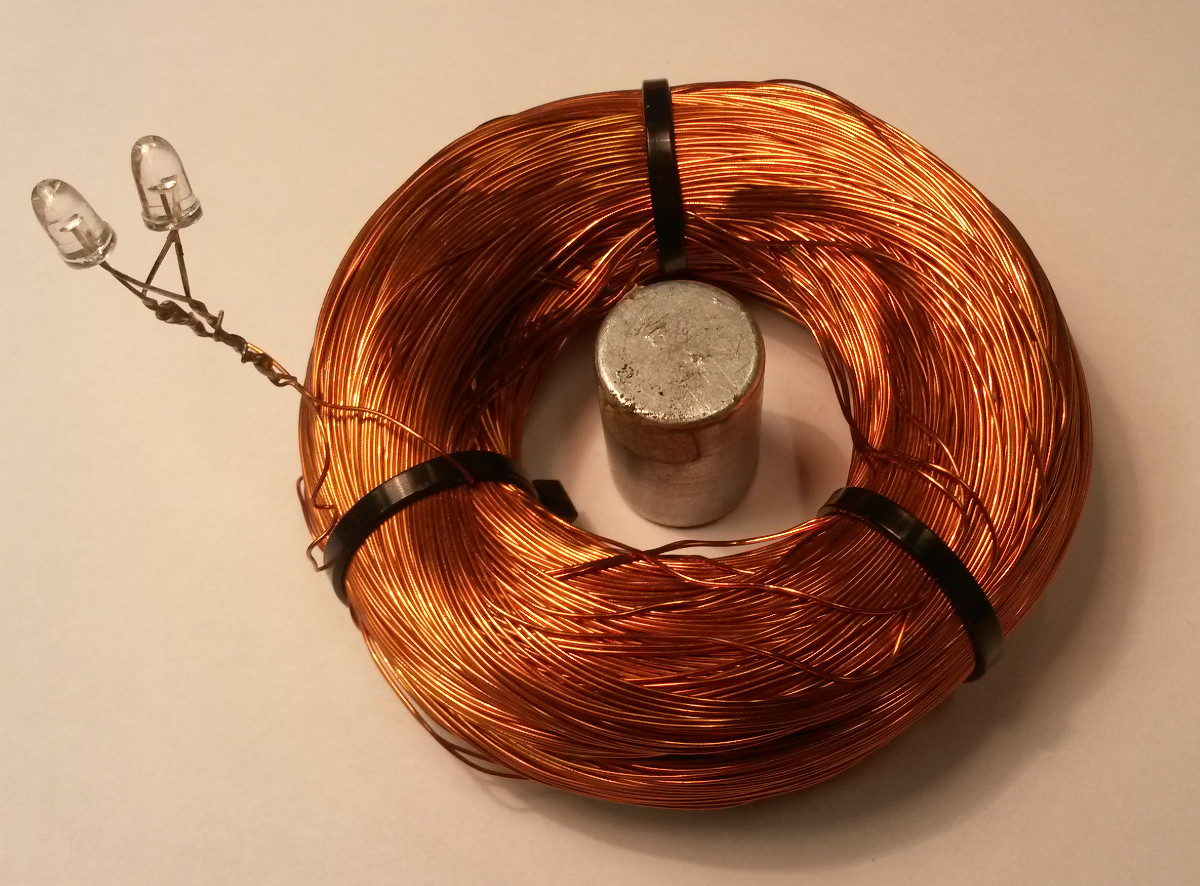
\includegraphics[height=55mm]{./ledspole.jpg}
	\caption{Tämä on esimerkki kuvatekstistä.}
	\label{kuv:kela}
\end{figure}

\begin{figure}[htb]
	\centering
	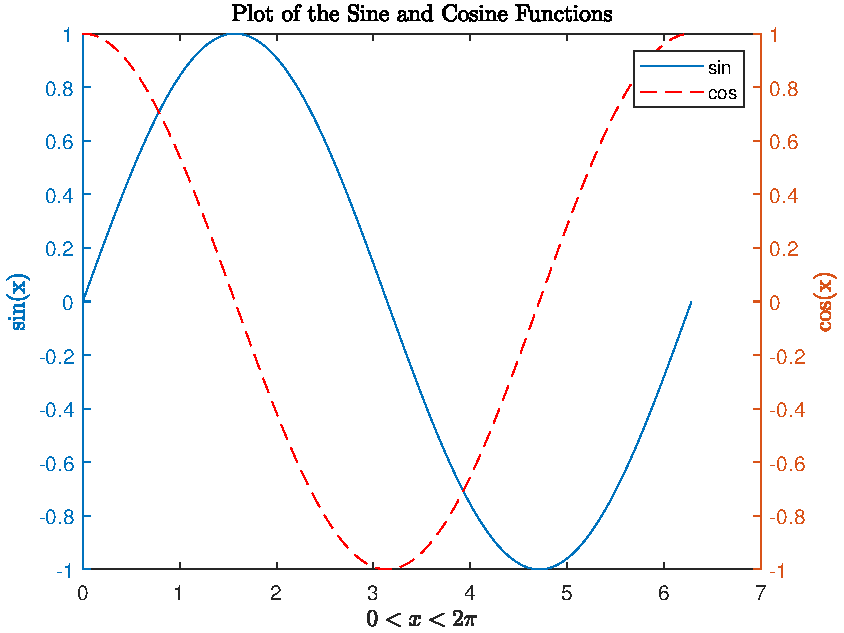
\includegraphics[height=6cm]{curves.pdf}
	%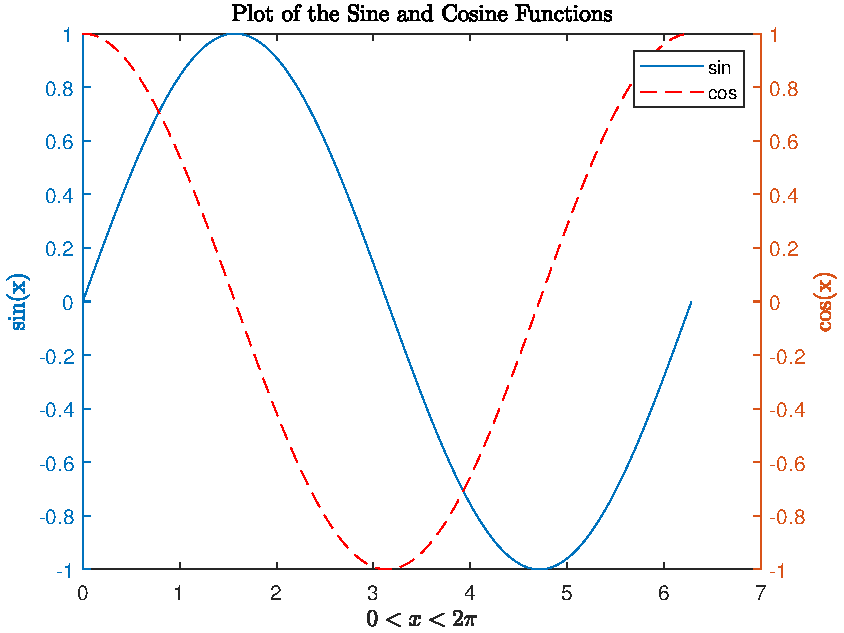
\includegraphics[height=5cm]{curves.eps}
	\caption{Tämä on esimerkki MATLAB-kaaviokuvasta. \label{kuv:matlab}}
\end{figure}

%% Esimerkki taulukosta
\begin{table}[htb]
	\caption{\label{tau:eläimet}Esimerkkitaulukko. Yleisiä eläimiä luokkansa
		mukaan.}
	\begin{center}
		\begin{tabular}{c|c|c}
			\hline
			\textbf{Nisäkkäät} & \textbf{Linnut} & \textbf{Hyönteiset}\\ \hline
			koira & varis & leppäkerttu \\ \hline
			kissa & varpunen & muurahainen \\ \hline
			rotta & tiainen & torakka \\ \hline  
		\end{tabular}
	\end{center}
\end{table}

Viittauksen kohteena oleva kuva tai taulukko tulisi mahdollisuuksien mukaan 
laittaa samalle sivulle, jolla siihen viitataan. Jos se on hankalaa, kuvan tai 
taulukon voi laittaa seuraavalle sivulle, mutta ei kauemmaksi. Useimmiten 
\LaTeX{} sijoittaa kuvat ja taulukot onnistuneesti, mutta joskus joudut 
ohjaamaan niiden sijoittelua \texttt{figure} ja \texttt{table} -ympäristöjen 
parametreillä \texttt{b} (bottom), \texttt{h} (here), \texttt{t} (top) ja 
\texttt{p} (page) ja mahdollisesti hieman säätämällä kuvien kokoa. Kuvien ja 
taulukoiden sijoittaminen lähelle viittausta voi olla mahdotonta, jos kuvia on 
paljon.

Taulukoita tai kuvia ei tulisi asemoida niin, että niiden jälkeen tai niitä 
ennen tulee vain yksi tai kaksi riviä, koska yksittäiset rivit saattavat olla 
vaikeita hahmottaa kuvien seasta tai ne voivat jäädä huomaamatta. Jos kahden 
kuvan välissä olisi muutoin vain vähän tekstiä, kuvat voidaan sijoittaa sivun 
yläreunaan, ja teksti voi tulla niiden jälkeen. Toinen vaihtoehto olisi laittaa 
teksti sivun yläosaan ja kuvat niiden jälkeen tai asetella kaikki teksti 
keskelle ja yksi kuva sen yläpuolelle ja toinen alapuolelle. Asettelun pitäisi 
olla mahdollisimman helppolukuinen --- kuvien sisältö vaikuttaa tähän. Lisäksi 
sivun tulisi näyttää siistiltä ja miellyttää silmää.

\subsection{Opinnäytteen osiin viittaaminen}

\LaTeX{}:ssa dokumentissa numeroituun osaan (lukuun, kuvaan, taulukoon, 
kaavaan jne.) viittaaminen on hyvin suoraviivaista. Numeroidun elementtiin 
liitetään ainutkertainen tunnistenimi käskyllä \verb+\label{nimi}+ ja haluttuun 
numeroituun osaan viitataan käskyllä \verb+\ref{nimi}+. Ole järjestelmällinen 
nimetessä dokumentin eri osia. Esimerkiksi aloita kuvan tunnistenimi merkeillä 
\texttt{kuv:}, taulukon merkeillä \texttt{tau:}, kappaleen merkeillä 
\texttt{luk:} ja kaava merkeillä \texttt{eq:}, kuten tässä mallipohjassa on 
tehty. Siten dokumentissa voi olla tunnistenimet \verb+\label{luk:Ohminlaki}+, 
\verb+\label{eq:Ohminlaki}+, \verb+\label{kuv:Ohminlaki}+ ja 
\verb+\label{tau:Ohminlaki}+.

Huomaa, että kuva- ja taulukko-sana kirjoitetaan pienellä ristiviitteessä. 
Ristiviitteissa usein näkee myös käytettävän sanat isolla kirjaimella kuten 
Kuva ja Taulukko. Mikä tahansa kirjoitusasu valitaankin selitteisiin --- 
taulukoihin, kuviin, kappaleisiin tai kaavoihin --- valittua kirjoitusasua 
tulee käyttää johdonmukaisesti. Sido ristiviitteen sana sen tunnistenimeen 
tilde-merkillä ettei \LaTeX{} taita ne eri riville. Viitatessasi lukualueeseen, 
kuten useampaan lukuu tai kaavaan, käytä endash -viivaa (\verb+--+). Esimerkki: 
Luvut~\ref{luk:johdanto}--\ref{luk:yhteenveto}\ldots

Viitataaksesi tiettyyn lukuun kirjoita luvun tunnistenimi heti luvun 
otsikkomäärittelyn perään ja viittaa kyseiseen lukuun seuraavasti:
%% verbatim -ympäristössä teksti ladotaan sellaisenaan. Käskyjä ei tulkita ja
%% siten tekstiä ei ladotan käskyjen määrämällä tavalla.
\begin{verbatim}
	\subsection{Ohmin laki}
	\label{luk:Ohminlaki}
	...
	...kuten luvussa~\ref{sec:ohmslaw} on esitetty, vastus...
\end{verbatim}
Sanan 'luvussa' ja tunnistenimen '\verb+\ref{sec:ohmslaw}+' välissä oleva 
tilde-merkki sekä latoo normaalinkokoisen välilyönnin että sitoo tunnistenimeen 
liittyvän luvun sanaan 'luvussa' niin, että niitä ei ladota eri riville, jos ne 
esiintyvät rivin lopussa. Käytä aina tilde-merkkiä tunnistesanan ja 
tunnistenimen välissä.

Kuvissa ja taulukoissa kirjoita tunnistenimen \verb+caption+-makron jälkeen. 
Yksinkertaisissa kaavoissa kirjoita tunnistenimen \verb+\begin{equation}+:in
perään. Voit viitata yksittäiseen kaavaan kuten kaavaan tai 
yhtälöön~\ref{eq:ohm1} tai koko yhtälöryhmään~\ref{eq:ohm} laittamalla 
\verb+\label+ -tunniste sopivasti.

\subsection{Lähteisiin viittaaminen}

Lähdeviittaukset tulee tehdä huolellisesti ja johdonmukaisesti
numeroviitejärjestelmän mukaisesti. Numeroviitteet järjestetään lähdeluetteloon 
viittausjärjestykseen, mutta jos lähdeluettelo on hyvin laaja (useita sivuja), 
järjestetään viitteet pääsanan mukaiseen aakkosjärjestykseen. 
Alaviitejärjestelmää\footnote{Myöskään alaviitteenä olevia kommentteja 
\underline{ei} suositella käytettäviksi.} ei käytetä. Liite~\ref{liite:viitteet}
käsittelee viitausjärjestelmät, viittaminen ja lähdeluettelon laatimista 
seikkaperäisesti. 

\subsection{Lähdeluettelo} 

Lähdeluettelossa esiintyy tavallisesti seuraavassa esitettäviä lähteitä, joista 
on numeroviitejärjestelmässä ilmoitettava asianomaisessa kohdassa vaaditut 
tiedot. Liitteessä~\ref{liite:viitteet} kuvataan yksityiskotaisesti, miten 
erilaisia lähteitä asemoidaan lähdeluettelossa. Kattava lista eri lähdetyypeistä 
löytyy Aalto-yliopiston verkkosivulta \cite{aaltolib}.\\

\noindent
\textit{Kirjasta} ilmoitetaan seuraavat tiedot:
\begin{itemize}
\setlength{\itemsep}{-3pt}
	\item[--]tekijät 
	\item[--]julkaisun nimi
	\item[--]painos, jos useita
	\item[--]kustannuspaikka
	\item[--]julkaisija tai kustantaja
	\item[--]julkaisuaika
	\item[--]mahdollinen sarjamerkintö. 
\end{itemize}
Viitteet \cite{Kauranen}--\cite{Koblitz} ovat esimerkkejä kirjan esittämisestä 
lähdeluettelossa. Viite \cite[s.\ 83--124]{Koblitz} on esimerkki 
lähdeluettelossa esiintyvän kirjan tiettyjen sivujen esittämisestä tekstissä.

\noindent
\textit{Artikkelista} kausijulkaisussa ilmoitetaan seuraavat tiedot:
\begin{itemize}
\setlength{\itemsep}{-3pt}
	\item[--]tekijät
	\item[--]artikkelin nimi
	\item[--]kausijulkaisun nimi
	\item[--]julkaisuvuosi
	\item[--]kausijulkaisun volyymi tai ilmestymisvuosi
	\item[--]kausijulkaisun numero
	\item[--]sivut, joilla artikkeli on.
\end{itemize}
Viitteet \cite{bcs}--\cite{Deschamps} ovat esimerkkejä artikkelin esittämisestä 
lähdeluettelossa.

\noindent
\textit{Kokoomateoksen luvusta tai osasta} ilmoitetaan seuraavat tiedot:
\begin{itemize}
	\setlength{\itemsep}{-3pt}
	\item[--]luvun tai osan tekijät
	\item[--]luvun tai osan nimi
	\item[--]maininta ``Teoksessa´´
	\item[--]koko teoksen toimittajat sekä maininta ``(toim.)´´
	\item[--]koko teoksen tai konferenssin nimi
	\item[--]konferenssiesitelmän kyseessä ollessa sen pitopaikka ja -aika
	\item[--]painos, jos useita
	\item[--]kustannuspaikka
	\item[--]julkaisija tai kustantaja, jos aihetta tämän ilmoittamiseen on
	\item[--]julkaisuaika
	\item[--]sivut, joilla luku tai osa on 
	\item[--]mahdollinen sarjamerkintä.
\end{itemize}
Viitteet \cite{Sihvola}--\cite{Lindblom} ovat esimerkkejä kokoomateoksen luvun 
tai osan esittämisestä lähdeluettelossa. 

\noindent
\textit{Opinnäytetyöstä} ilmoitetaan seuraavat tiedot:
\begin{itemize}
	\setlength{\itemsep}{-3pt}
	\item[--]tekijä
	\item[--]työn nimi
	\item[--]opinnäytetyön tyyppi
	\item[--]oppilaitoksen nimi
	\item[--]osaston, laitoksen tai ohjelman nimi
	\item[--]oppilaitoksen sijaintipaikka
	\item[--]vuosiluku.
\end{itemize}
Viitteet \cite{Miinusmaa}--\cite{Lonnqvist} ovat esimerkkejä opinnäytteen 
esittämisestä lähdeluettelossa. 

\noindent
\textit{Standardista} ilmoitetaan seuraavat tiedot:
\begin{itemize}
	\setlength{\itemsep}{-3pt}
	\item[--]standardin tunnus ja numero
	\item[--]standardin nimi
	\item[--]painos, mikäli ei ole ensimmäinen
	\item[--]julkaisupaikka
	\item[--]julkaisija
	\item[--]julkaisuvuosi
	\item[--]sivumäärä.
\end{itemize}
Viite \cite{sfs} on esimerkki standardin esittämisestä opinnäytteen
lähdeluettelossa. 

\noindent
\textit{Haastattelusta} ilmoitetaan seuraavat tiedot:
\begin{itemize}
	\setlength{\itemsep}{-3pt}
	\item[--]haastatellun henkilön nimi
	\item[--]haastatellun henkilön arvo tai asema
	\item[--]haastatellun henkilön edustama organisaatio
	\item[--]organisaation osoite
	\item[--]maininta siitä, että kyseessä on haastattelu ja haastattelun
	päivämäärä. 
\end{itemize}
Viite \cite{haastattelu} on esimerkki haastattelun esittämisestä 
lähdeluettelossa.

\noindent
Osa sähköisessä muodossa olevista artikkeleista on saatavissa myös
painettuina. \textit{Vain verkosta saatavissa olevasta artikkelista} esitetään
seuraavat tiedot:
\begin{itemize}
	\setlength{\itemsep}{-3pt}
	\item[--]tekijät
	\item[--]artikkelin nimi
	\item[--]kausijulkaisun nimi
	\item[--]viestintyyppi
	\item[--]laitos tai volyymi
	\item[--]kausijulkaisun yksittäistä osaa koskeva merkintä tai numero
	\item[--]julkaisuvuosi tai maininta >>Päivitetty>> ja päivitysaika
	\item[--]maininta >>Viitattu>> ja viittaamisen ajankohta 
	\item[--]maininta >>Saatavissa>> ja URL tai 
	maininta >>DOI>> ja DOI-numero (DOI=Digital Object Identifier).
\end{itemize}
Viitteet \cite{Ribeiro}--\cite{kone} ovat esimerkkejä sähköisessä muodossa 
olevan artikkelin esittämisestä opinnäytteen lähdeluettelossa. Viitteet 
\cite{Ribeiro} ja \cite{Stieber} ovat saatavissa sekä painettuna että verkosta, 
joten viitteiden esitystapa mukailee painetun artikkelin viitteen esitystapaa, 
mutta sen lisäksi kerrotaan julkaisun olevan verkkolehti ja lehden olevan 
saatavissa myös painettuna.  Viite \cite{kone} on saatavissa vain verkosta ja
siitä esitetään yllä vaaditut tiedot. Valitettavasti sähköisessä muodosssa 
olevasta artikkelista ei ole aina saatavissa lai\-tos-, volyymi- tai 
numerotietoja.

\noindent
\textit{Sähköisessä muodossa olevasta opinnäytetyöstä} ilmoitetaan
seuraavat tiedot:
\begin{itemize}
	\setlength{\itemsep}{-3pt}
	\item[--]tekijä
	\item[--]työn nimi
	\item[--]viestintyyppi
	\item[--]opinnäytetyön tyyppi
	\item[--]oppilaitoksen nimi
	\item[--]osaston, laitoksen tai ohjelman nimi
	\item[--]oppilaitoksen sijaintipaikka
	\item[--]vuosiluku
	\item[--]viittamisen ajankohta
	\item[--]maininta "Saatavissa" ja URL tai 
	maininta "DOI" ja DOI-numero.
\end{itemize}
Viite \cite{Adida} on esimerkki sähköisessä muodossa olevan opinnäytteen 
esittämisestä lähdeluettelossa.

\noindent
Viite \cite{viittaaminen} on esimerkki itsenäisen kirjoituksen sisältävästä
verkkosivusta. Tällainen lähde on rinnastettavissa erillisteokseen.
\textit{Verkkosivusta} esitetään tiedot:
\begin{itemize}
	\setlength{\itemsep}{-3pt}
	\item[--] tekijät
	\item[--] otsikko
	\item[--] maininta "Päivitetty" ja päivitysaika 
	\item[--] maininta "Viitattu" ja viittaamisen ajankohta
	\item[--] Maininta "Saatavissa" ja URL.
\end{itemize}
Joskus verkkosivun kirjoitus on jaettu useammalle sivulle, jolloin
lähdeluetteloon kirjataan vain sellainen verkko-osoite, joka koskee koko 
kirjoitusta tai sen etusivua, ellei sitten todella tarkoiteta kirjoituksen 
yksittäistä sivua. 


%% Opinnäytteessä jokainen osa alkaa uudelta sivulta, joten \clearpage
%%
\clearpage
\section{Tutkimusaineisto ja -metodit}

Tämä on opinnäytteen ydinosa, jossa kerrotaan metodologiset valinnat ja niiden 
rajoitteet, tutkimusaineiston tai tutkittavien henkilöiden valintaperiaatteet, 
tutkimuksen toteutus ja käytetyt metodit. Tässä osassa tulevat esiin 
opinnäytteen vahvuudet ja heikkoudet. Taustatiedoksi metodista riittää tieto 
siitä, miten muut tutkijat ovat sitä aiemmin käyttäneet. Opinnäytteessä tulee 
keskittyä opinnäytteen tekijän omiin saavutuksiin.

Kirjallisuustutkielmissa ei ole erillistä lukua aineistosta ja metodeista. Sen 
sijaan teoreettinen käsittely jaetaan lukuihin yleensä asiakokonaisuuksien tai 
näkökulmien mukaan.


%% Opinnäytteessä jokainen osa alkaa uudelta sivulta, joten \clearpage
%%
\clearpage
\section{Tulokset}

Tässä luvussa esitellään empiirisen tai taiteellisen työn tulokset ja vastataan 
tutkimuskysymyksiin, jotka on esitetty aiemmin, esimerkiksi johdannossa. Työn 
tieteellinen arvo mitataan saaduilla tuloksilla ja sillä, miten hyvin 
argumentointi tukee tutkimuskysymyksiin vastaamista. Kirjallisuustutkielmissa 
ei tyypillisesti ole erillistä päälukua tuloksille, vaan päätelmät, niiden 
arviointi ja merkitys kootaan yhteenvetolukuun.

Omien tulostensa merkitsevyyteen tulee suhtautua kriittisesti. Tuloksiaan ja 
omaa tulkintaansa niistä voi tarkastella kriittisesti joko tässä luvassa tai 
sitten myöhemmässä, tarkastelun tai johtopäätökset sisältävässä luvussa. 

Tässä osassa tulisi käsitellä tutkimuksessa käytetyn aineiston luotettavuutta. 
Johtopäätöksien luotettavuutta voi käsitellä joko tässä luvussa tai myöhemmässä 
tarkasteluosassa. Asiaa voi käsitellä omassa luvussaan eril-lään yhteenvedosta 
tai johtopäätöksistä.


%% Opinnäytteessä jokainen osa alkaa uudelta sivulta, joten \clearpage
%%
\clearpage
\section{Yhteenveto/Johtopäätökset}
\label{luk:yhteenveto}

Tässä luvussa vedetään kaikki yhteen. Yhteenvedossa kerrotaan lukijalle 
lyhyesti ja selkeästi, mitä on tehty ja saatu selville sekä mikä on tulosten 
arvo suhteessa vastaavaan aiempaan tutkimukseen. Tutkimuskysymyksestä, 
alakysymyksistä ja hypoteeseista pitää tehdä selkeitä johtopäätöksiä. Tässä 
luvussa voidaan myös keskustella tulevista tutkimusmahdollisuuksista ja 
tutkimuskysymyksistä, joita olisi voitu esittää.

Opinnäytteen tekijä on vastuussa siitä, että opinnäytteen ulkoasu, muoto ja 
rakenne vastaavat oman korkeakoulun ohjeita. Mallipohjan tarkoitus on auttaa 
täyttämään annetut vaatimukset.



\clearpage
%% Lähdeluettelo
%%
\thesisbibliography

\begin{thebibliography}{99}
	
%% Tässä likainen temppu jolla saa tekstiä lähdeluettelon otsikon ja ensimmäisen
%% lähteen väliin. Et tarvitse tätä opinnäytetyössäsi, joten poista tämä kohta.
\item[]
\hskip-\leftmargin
\begin{minipage}{\textwidth}
	Tässä on lista lähteistä joihin viitataan liitteessä~\ref{liite:asemointi}. 
	Listä suurin piirtein noudattaa Vancouver-viittausjärjestelmää.  
	Liitteessä~\ref{liite:viitteet} kerrotaan esimerkkein eri 
	viitausjärjestelmistä. Noudata siellä olevat ohjeet omassa työssäsi.
\end{minipage}
\bigskip
%% Likainen temppu päättyy.

%% Alla esimerkki englanninkielisen tavuttamisen pakottamisesta.
%% Oletusarvoisesti käytetään suomalaista tavutusta, mutta viitteissä
%% esiintyy usein muunkielisiä lauseita, jotka tulevat siten tavutetuksi
%% suomen kielen sääntöjen mukaan. Tämän voi korjata \foreignlanguage-
%% komennolla, jonka ensimmäinen parametri on vieraan kielen nimi ja toinen 
%% on vieraalla kielellä tavutettava teksti. 
\bibitem{aaltolib} \foreignlanguage{english}{Citation Guide: Making a 
	bibliography, \textit{Aalto University Learning Centre}}
 (verkkoaineisto) (viitattu 14.7.2021). 
 Saatavissa: \url{https://libguides.aalto.fi/c.php?g=410672&p=2796631} 

\bibitem{Bringhurst} \foreignlanguage{english}{Bringhurst, R.
	\textit{Horizontal Motion. The Elements of Typographic Style}, Point 
	Roberts, WA: Hartley \& Marks,} 1992. s.\ 26, 
 s.\ 25--36. (viitattu 7.5.2021). Versio 3.0 saatavissa myös verkossa: 
 \url{https://smallpressblog.files.wordpress.com/2017/11/bringhurstelementsselections1.pdf}

\bibitem{Unna} de Buen Unna, J. \foreignlanguage{spanish}{\textit{Manual de 
		dise\~no editorial}, 4. ed. corrigida y aumentada, Somonte-Cenero, 
	Gij\'on: Ediciones Trea, 2014.}

\bibitem{Dyson} \foreignlanguage{english}{Dyson, M. C., and Kipping, G. J. The 
	Effects of Line Length and Method of Movement on Patterns of Reading from 
	Screen. \textit{Visible Language,}} vol.~2, nro.~2, s.~150--181, 1998.

\bibitem{Shaik} Shaikh, A. D. \foreignlanguage{english}{The Effects of Line 
	Length on Reading Online News. \textit{Usability News}}, vol.~7, nro.~2, 
	heinäkuu 2005.

\bibitem{Bailey} Bailey, C. \foreignlanguage{english}{\textit{The Basics of 
		Typography}} (verkkoaineisto) (viitattu 14.7.2021). 
 \url{https://www.webfx.com/blog/web-design/the-basics-of-typography}

\bibitem{Wikilinelength} \foreignlanguage{english}{Wikipedia contributors, 
	''Line length''. \textit{Wikipedia: The Free Encyclopedia}, Wikimedia 
	Foundation, Inc. (2004)}
 (Verkkoaineisto) (viitattu 7.5.2021). 
 \url{https://en.wikipedia.org/w/index.php?title=Line_length&oldid=997524503}

\bibitem{enwiki:1026690618} \foreignlanguage{english}{Wikipedia contributors, 
	''Leading''. \textit{Wikipedia, The Free Encyclopedia}} (verkkoaineisto) 
 (viitattu 14.7.2021).
 \url{https://en.wikipedia.org/w/index.php?title=Leading&oldid=1026690618}

\bibitem{aaltovisual} Aalto-yliopiston visuaalinen ilme.
\textit{Aalto-yliopisto Brandiohjeisto}.
\url{https://www.aalto.fi/fi/brand-library#/visual-elements/typography}
(viitattu 14 July 2021)

%% Sama temppu vielä kerran
\bigskip
\item[]
\hskip-\leftmargin
\begin{minipage}{\textwidth}
	Alla oleva viiteluettelo sisältää esimerkkejä erilaisista lähteistä. 
	Luettelo suurin piirtein noudattaa Vancouver-viittausjärjestelmää. 
	Liittestä~\ref{liite:viitteet} löydät tarkempaa kuvausta viiteluettelon 
	laatimiseksi.
\end{minipage}
%\medskip
%%

\bibitem{Kauranen} Kauranen, I., Mustakallio, M. ja Palmgren, V. 
\textit{Tutkimusraportin kirjoittamisen opas opinnäytetyön tekijöille.} 
Espoo, Teknillinen korkeakoulu, 2006.

\bibitem{Itkonen} Itkonen, M. \textit{Typografian käsikirja.} 3. painos.
Helsinki, RPS-yhtiöt, 2007.

\bibitem{Koblitz} \foreignlanguage{english}{Koblitz, N. \textit{A Course in 
	Number Theory and Cryptography. Graduate Texts in Mathematics 114.}}
  2. painos. New York, Springer, 1994.

%% Kun on useampi nimikirjain, jokaisen nimikirjaimen väliin kuuluu
%% välilyönti. Oikea välin määrä on saatu \<välilyönnillä>.
%% Kun pisteen jälkeen seuraava merkki on iso kirjain, LaTeX katsoo uuden
%% virkkeen alkaneen ja lisää pistten jälkeen normaalia välilyöntiä hieman
%% pidemmän välin.
\bibitem{bcs} Bardeen, J., Cooper, L.\ N. ja Schrieffer, J.\ R.
   \foreignlanguage{english}{Theory of Superconductivity. 
   \textit{Physical Review,}} 1957, vol.~108, nro~5, s. 1175--1204.

\bibitem{Deschamps} Deschamps, G.\ A. \foreignlanguage{english}{
	Electromagnetics and Differential Forms. \textit{Proceedings of the IEEE,}} 
	1981, vol.~69, nro~6, s. 676--696.

\bibitem{Sihvola} Sihvola, A. et al.
	\foreignlanguage{english}{Interpretation of measurements of helix and bihelix 
		superchiral structures.}
Teoksessa: Jacob, A.\ F. ja	Reinert, J. (toim.)
\foreignlanguage{english}{\textit{Bianisotropics '98 7th International 
		Conference on Complex Media.}}
\foreignlanguage{german}{Braunschweig, 3.--6.6.1998. Braunscweig, Technische 
	Universität Braunschweig,} 1998, s. 317--320.

%% Alla on suomalainen yhdistelmäsukunimi. Sen nimien välissä käytetään
%% yhdysmerkkiä l. tavuviivaa, kirjoitetaan -.
\bibitem{Lindblom} Lindblom-Ylänne, S. ja Wager, M.
   Tieteellisten opinnäytetöiden ohjaaminen.
   Teoksessa: Lindblom-Ylänne, S. ja Nevgi, A. (toim.)
   \textit{Yliopisto- ja korkeakouluopettajan käsikirja.}
   Helsinki, WSOY, 2004, s. 314--325.

\bibitem{Miinusmaa} Miinusmaa, H. Neliskulmaisen reiän poraamisesta
   kolmikulmaisella poralla. Diplomityö, Teknillinen korkeakoulu,
   konetekniikan osasto, Espoo, 1977.

\bibitem{Loh} Loh, N.\ C. \foreignlanguage{english}{High-Resolution 
	Micromachined Interferometric Accelerometer. Master's Thesis, 
	Massachusetts Institute of Technology, Cambridge, Massachusetts,} 1992.

\bibitem{Lonnqvist} Lönnqvist, A.
   \foreignlanguage{english}{Applications of hologram-based compact range:
	antenna radiation pattern, radar cross section, and absorber reflectivity 
	measurements.}
	Väitöskirja, Teknillinen korkeakoulu, sähkö- ja tietoliikennetekniikan
	osasto, 2006.
	
\bibitem{sfs} SFS 5342. Kirjallisuusviitteiden laatiminen. 2. painos.
   Helsinki, Suomen standardisoimisliitto, 2004. 20~s.

\bibitem{haastattelu} Palmgren, V. Suunnittelija. Teknillinen korkeakoulu,
   kirjasto. Otaniementie 9, 02150 Espoo. Haastattelu 15.1.2007.

\bibitem{Ribeiro} Ribeiro, C.\ B., Ollila, E. ja Koivunen, V.
   \foreignlanguage{english}{''Stochastic Maximum-Likelihood Method for MIMO
	Propagation Parameter Estimation,''}
	\textit{IEEE Transactions on Signal Processing,} verkkolehti, vol.~55,
	nro~1, s. 46--55. Viitattu 19.1.2007. Lehti ilmestyy myös painettuna. 
	DOI: 10.1109/TSP.2006.882057.

\bibitem{Stieber} Stieber, T. GnuPG Hacks. \textit{Linux Journal,}
   verkkolehti, 2006, maaliskuu, nro~143. Viitattu 19.1.2007. Lehti ilmestyy
   myös painettuna. Saatavissa: \url{http://www.linuxjournal.com/article/8732.}

\bibitem{kone} Pohjois-Koivisto, T. Voiko kone tulevaisuudessa arvata tahtosi? 
   \textit{Apropos,} verkkolehti, helmikuu, nro~1, 2005. Viitattu 19.1.2007. 
Saatavissa: \url{http://www.apropos.fi/1-2005/prima.php.}

\bibitem{Adida} Adida, B. \foreignlanguage{english}{Advances in Cryptographic 
	Voting Systems.} Verkkodokumentti. 
	\foreignlanguage{english}{Ph.D.\ Thesis, Massachusetts Institute of	
		Technology, Cambridge, Massachusetts,} 2006. Viitattu 19.1.2007. 
	Saatavissa:
	\url{http://crypto.csail.mit.edu/~cis/theses/adida-phd.pdf.}

\bibitem{viittaaminen} Kilpeläinen, P. WWW-lähteisiin viittaaminen 
   tutkielmatekstissä. Verkkodokumentti. Päivitetty 26.11.2001.
   Viitattu 19.1.2007. Saatavissa:
   \url{http://www.cs.uku.fi/~kilpelai/wwwlahteet.html.}

\end{thebibliography}


%% Liitteet
%% Jos liiteitä ei ole, poista a.o. \clearpage- ja \thesisappendix -makrot sekä 
%% kaikki sitä seuraava teksti.
\clearpage
\thesisappendix

\section{Liitteen sisältö}
\label{liite:sisalto}

Liitteet eivät ole opinnäytteen kannalta välttämättömiä. Kirjoittaessa 
opinnäytettäsi on hyvä ajatella pärjääväsi ilman liitteitä. Älä paisuta turhaan 
liitteitä pitääksesi tekstiosan pituuden annetuissa rajoissa. Tällä tavalla ei 
synny hyvää opinnäytettä.   

Liite on itsenäinen kokonaisuus, vaikka se täydentääkin tekstiosaa. Liite ei 
siten ole pelkkä listaus, kuva tai taulukko, vaan liitteessä selitetään aina 
sisällön laatu ja tarkoitus. Liitteeseen voi laittaa esimerkiksi listauksia. 
Alla on yksinkertaistettu listausesimerkki tämän liitteen luomisesta. 
%% Verbatim-ympäristö ei muotoile tai tavuta tekstiä. Fontti on monospace.
%% Verbatim-ympäristön sisällä annettuja komentoja ei LaTeX käsittele. 
%% Vasta \end{verbatim}-komennon jälkeen jatketaan käsittelyä.
\begin{verbatim}
	\clearpage
	\appendix
	\addcontentsline{toc}{section}{Liitteen sisältö}
	\thispagestyle{empty}
	\section*{Liitteen sisältö}
	...
	tekstiä
\end{verbatim}

Kaavojen numerointi muodostaa liitteissä oman kokonaisuutensa. Tässä pari 
esimerkkiä, miten mahdolliset liitteessä olevat kaavat numeroidaan:
\begin{align}
	(x+a)^n &= \sum_{k=0}^n \binom{a}{b} x^n a^{n-k}, \label{appeq:1}\\
	\sin\alpha \pm \sin\beta &= 2\sin\left(\frac{\alpha\pm\beta}{2}\right)
	\sin\left(\frac{\alpha\mp\beta}{2}\right). \label{liitekaava2}
\end{align}

Liiteeseen voi sisältää kuvia jotka eivät istu varsinaisen työn tekstiin mutta 
täydentävät sitä. Liitteen kuvat numeroidan samalla tavalla kuin kaavat: katso
kuvaa~\ref{liitekuv:taitto}.

\begin{figure}[b]
	\centering
	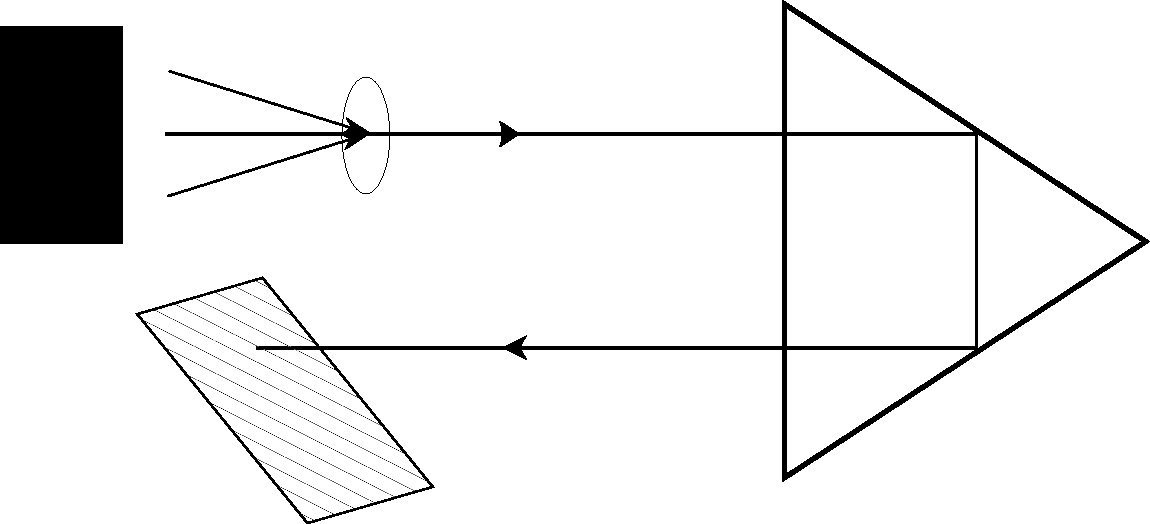
\includegraphics[height=31mm]{./linediagram.pdf}
	\caption{Tämä on esimerkki liitteessä numeroidun kuvan kuvatekstistä. 
		\label{liitekuv:taitto}}
\end{figure}

Liitteiden taulukoiden numerointi on kuvien ja kaavojen kaltainen, esimerkkinä taulukko~\ref{liitetau:aikataulu}:
\begin{table}[htb]
	\centering
	\caption{Taulukon kuvateksti. \label{liitetau:aikataulu}}
	\sffamily% change the font in the table to sans serif
	\fbox{
		\begin{tabular}{lp{0.5\linewidth}}
%			9.00--9.55  & Safety instructions on the use of laboratories\\
%			9.55--10.00 & Transfer to the laboratory
			9.00--9.55  & Käytettävyystestauksen tiedotustilaisuus
				(valmistautumistehtävät annettu).\\
			9.55--10.00 & Testausalueelle siirtyminen
	\end{tabular}}
\end{table}


\clearpage
\section{Sivun asettelu ja typografinen suunnittelu}
\label{liite:asemointi}

\subsection*{Aalto-yliopiston ohjeet opinnäytteiden ulkoasulle}

Aalto-yliopiston visuaaliseen ohjeistukseen asiakirjojen kirjoittamisesta 
viite \cite{aaltovisual} liittyy fontteja koskeva ohjeistus. Tässä ohjeessa 
tarkennetaan, että leipätekstissä käytetään pääteviivallista Sentinel-fonttia ja
lukujen otsikoissa pääteviivatonta Nimbus Sans -fonttia lihavoituna. Nämä fontit 
pitäisi olla asennettuna kaikille Aallon koneille. Koska kyseessä on kaupallinen 
tuote, Sentinelin voi korvata opinnäytteessä Georgialla ja Nimbus Sansin 
Arialilla, jotka molemmat löytyvät asennettuina kaikilta Windows-koneilta. 
Yliopiston tarjoamassa Woed-pohjassa käytetään Georgiaa ja Arialia. Tässä 
pohjassa käytetään \verb+newtxtext+ -paketista löytyvät Times- sekä 
Helvetica-fonttien klooneja, koska paketti tarjoa yhteensopivaa 
matematiikka-fonttia ja \LaTeX:in tuottama pdf-tiedosto on PDF/A-standardin 
mukainen pdf-tiedosto.

\subsection*{Sivun asettelu ja typografiset määrittelyt}
\subsubsection*{Opinnäytteen sivun asettelu}

Tässä opinnäytepohjassa on sivujen asetukset laitettu valmiiksi. Omia asetuksia
ei ole tarpeen laittaa. Tiedoksi kuitenkin periaatteet: Opinnäyte painetaan 
A4-kokoiselle paperille. leipätekstissä käytetyn fontin koko on 12\,pt. 
Verkkoversiossa teksti keskitetään siten, että kummankin reunan marginaali on 
3,4\,cm. Jos haluat tulostaa työn ja sitoa sen, sidonnan puolen marginaalin 
tulee olla 4,8\,cm. Tekstipalstan korkeudeksi asetetaan 23\,cm asettamalla 
ylämarginaaliksi 3,7\,cm ja alamarginaaliksi 3\,cm. Sivun asettelun mitat on 
koottu taulukkoon~\ref{liitetau:asemointi}.

\begin{table}[htb]
	\centering
	\caption{Otsikossa, lukujen otsikossa ja leipätekstissä käytetyt fontit ja fonttikoot.}
	\label{liitetau:asemointi}
	\sffamily% muuta taulukon fontti sans serif:ksi
	\begin{tabular}{ll}
		\hline
		Paperin koko & A4\\\hline
		Rivin pituus & 14,2\,cm \\\hline
		Ylämarginaali & 3,7\,cm \\\hline
		Alamarginaali & 3,0\,cm \\\hline
		\textbf{Verkkojulkaisu} & \\\hline
		Vasen marginaali & 3,4\,cm \\\hline
		Oikea marginaali & 3,4\,cm \\\hline
		\textbf{Tulostettu asiakirja} & \textbf{(sidottava versio)} \\\hline
		Vasen marginaali & 4,8\,cm \\\hline
		Oikea marginaali & 2,0\,cm \\\hline
	\end{tabular}
\end{table}

\subsubsection*{Leipäteksti ja tekstin jakaminen lukuihin}

Leipätekstissä käytetään fonttina Times-kloonia pistekoossa 12 ja lukujen 
otsikoissa lihavoitua Helvetica-klooni-fonttia. Opinnäytteessä tulee käyttää 
korkeintaan kolmea otsikkotasoa: luku, alaluku ja alaluvun alaluku. Alalukujen 
numerointi jatkuu ylätason numeroinnista. Esimerkiksi numero 2.1.3 viittaa 
luvun~2 alaluvun~1 alalukuun~3.

\clearpage
\section{Lähdeviitteet ja tekstiviitteet}
\label{liite:viitteet}
\subsection*{Viittausjärjestelmät}

Tämä mallipohja ohjaa suomenkieliseen kirjoittamiseen, vaikka suurin osa 
esimerkeistä alla onkin englanninkielisiä.

Lähteisiin viittaaminen tekstissä (tekstiviitteet) on tiedeyhteisössä 
vakiintunut tapa, jolla kirjoittaja osoittaa lainaavansa toisen tekstiä tai 
ajatuksia joistakin tietyistä lähteistä. Jokaisen lähteen täydellisen 
lähdeviitteen tulee sisältyä lähdeluetteloksi nimettyyn osioon.

Tieteellisessä kirjoittamisessa on kaksi pääasiallista viittausjärjestelmää: 
Harvard-järjestelmä ja Vancouver-järjestelmä. Harvard-järjestelmästä on tullut 
yläkäsite kaikille järjestelmille, joissa ilmoitetaan tekijän nimi ja vuosi 
(kuten APA-järjestelmässä) tai tekijän nimi ja sivunumero (kuten 
MLA-järjestelmässä) sulkeiden sisällä. Harvard-järjestelmää käytetään edelleen 
jonkin verran luonnontieteissä (esim. American Chemical Society, 2006). Se on 
käytetyin viittaustapa yhteiskuntatieteissä (esim. American Psychological 
Association, 2010), taiteen alalla sekä humanistisissa tieteissä (esim. Modern 
Languages Association, 2016; University of Chicago Press, 2017).

Vancouver-järjestelmä on nykyään laajasti käytössä insinöörialoilla sekä 
tekniikan ja perustieteiden aloilla. Järjestelmän tyypillinen piirre on 
tekstiviitteiden numerointi, ja sitä kutsutaankin myös 
numeroviitejärjestelmäksi. Yksi tärkeimmistä Vancouver-järjestelmän soveltajista
on IEEE Reference Guide (IEEE 2018). Vancouver-järjestelmässä tekstissä käytetty 
viitenumerointi vastaa numeroitua täydellistä lähdeluetteloa tekstin lopussa. 
Yleensä viitteet numeroidaan siinä järjestyksessä, kun ne esiintyvät ensi kertaa 
tekstissä. Sen jälkeen niihin viitataan koko ajan samalla numerolla. Vähemmän 
käytetyssä muunnelmassa tästä järjestelmästä lähteet numeroidaan tekijän mukaan 
aakkosjärjestykseen (ns. aakkosnumerojärjestelmä).

On olemassa myös kolmas, alaviitteisiin ja lähdeluetteloon perustuva 
järjestelmä. Se on toinen Chicago Manual of Stylen tyyleistä; toinen on tekijän 
nimeen ja vuoteen perustuva järjestelmä. Alaviitteisiin ja lähdeluetteloon 
perustuvaa järjestelmää käytetään lähinnä kirjallisuuden ja historian aloilla 
sekä joskus taiteissa, mutta sen käyttö on huomattavasti vähäisempää kuin 
Harvard-järjestelmän. Aaltodocissa olevista 97 englanninkielisestä 
väitöskirjasta (tilanne 5.3.2020) vain 14 väitöskirjassa käytettiin 
alaviitejärjestelmää. Koska alaviitejärjestelmän käyttö on Aallossa melko 
harvinaista, on viisainta katsoa ohjeita siihen Chicago Manual of Style 
-kirjoitusoppaasta.

Eri järjestelmissä käytetään välimerkkejä eri tavoin tekijän nimen, vuoden ja 
sivunumeron välissä (vrt. esim the Chicago Manual of Style (University of 
Chicago Press, 2017), the Publication Manual of the American Psychological 
Association (APA, 2018), the MLA Handbook (MLA, 2016) ja the New Oxford Style 
Manual (OUP, 2016)). Tärkeintä viittausjärjestelmän valinnassa on valinnasta 
sopiminen ohjaajan kanssa heti kirjoitusprosessin alussa ja valitun järjestelmän
käyttö johdonmukaisesti koko opinnäytteessä. Opinnäytteen valvoja voi antaa 
neuvoja alan tyypillisistä viittauskäytännöistä.

Alla on esitelty yleisiä ohjeita kahdesta pääasiallisesta viittausjärjestelmästä
niihin perehtyneiden kirjoitusoppaiden valossa. Viittausesimerkit on annettu 
tässä oppaassa kehystettynä selvyyden vuoksi, mutta kehyksiä ei tule käyttää 
opinnäytteessä.


\subsection*{Suora lainaus}

Kun lähdettä lainataan sanasta sanaan, lainaus merkitään kokolainausmerkkeihin 
(” ”) ja sen perään merkitään tekijän nimi, teoksen vuosi ja sivunumero 
sulkuihin (Harvard-järjestelmässä) tai viitteen numero hakasulkeisiin 
(Vancouver-järjestelmässä). On huomattava, että suorien lainausten käyttö 
vaihtelee eri tieteenaloilla: taiteen, suunnittelun ja arkkitehtuurin ja 
kauppatieteiden aloilla se on melko tavallista, mutta perustieteissä ja 
insinöörialoilla harvinaista. Siksi on hyvä kysyä ohjaajalta tai tarkistaa 
tunnetuista oman alan tieteellisistä julkaisuista, miten suoriin lainauksiin 
suhtaudutaan opinnäytteen alan asiantuntijoiden keskuudessa.


\subsubsection*{Suora lainaus Harvard-järjestelmän mukaan}

\newcounter{example}[section]
\refstepcounter{example}
\textsf{\textbf{Esimerkki~\theexample:}} Sisältöpainotteinen lainaus American Sociological Associationin (2019) mallin mukaan

\vspace{1ex}
\noindent
\fbox{\parbox{\textwidth-2\fboxsep}{\textsf{
			Attending to these breakdowns not only result in an on-going re-constitution
			of relations between people and things but are also hotbeds for unleashing 
			everyday “creativity, invention, imagination, and artfulness” (Jackson, 
			2014: 226).
}}}

\vspace{1ex}
\noindent
\textit{Lähde:} Durrani, M. 2018. Designers by any other name: exploring the 
sociomaterial practices of vernacular garment menders. \textit{Design Research 
	Society International Conference: Catalyst. DRS International Conference 
	Series.} 4: 1731-1746. ISBN 978-1-912294-19-0 (electronic). 
DOI: 10.21606/dma.2018.495. \copyright{} 2018 Design Research Society. Työ on  
Creative Commons Nimeä-EiKaupallinen-JaaSamoin 4.0 Kansainvälinen (CC BY-NC-SA 
4.0) - lisenssin alainen. 
\url{https://creativecommons.org/licenses/by-nc-sa/4.0/.}

\vspace{1em}
\noindent
\refstepcounter{example}
\textsf{\textbf{Esimerkki~\theexample:}} Tekijäkeskeinen lainaus American Psychological Associationin (2010) mallin mukaan

\vspace{1ex}
\noindent
\fbox{\parbox{\textwidth-2\fboxsep}{\textsf{
	Philosopher Mark Johnson (2007) argued that meanings emerge from “deeper 
	explorations into the qualities, feelings, emotions, and bodily processes” 
	(p. x).
}}}

\vspace{1ex}
\noindent
\textit{Lähde:} Aktaş, B. \& Mäkelä, M. (2019). Negotiation between the maker 
and material: Observations on material interactions in felting studio. 
\textit{International Journal of Design}, 13(2): 55--67. \copyright{} 
\textit{2019 Aktaş \& Mäkelä. Artikkelin tekijänoikeudet kuuluvat 
	kirjailijoille, ensijulkaisuoikeus International Journal of Designille. 
	Kaikki julkaisun sisältö, jollei toisin mainita, on Creative Commons 
	Nimeä-EiKaupallinen-EiMuutoksia 2.5 Yleinen (CC BY-NC-ND 2.5) -lisenssin 
	alaista.}


\subsubsection*{Sisennetty lainaus}

Pitkät lainaukset sisennetään omaksi kappaleekseen. On syytä huomioida, että 
kaikki lainaukseen kuuluvat lauseet sisennetään eikä lainausmerkkejä käytetä. 
Joka viittausjärjestelmällä on oma määritelmänsä siitä, minkä pituinen lainaus 
sisennetään omaksi kappaleekseen: AMA suosittelee mini-mipituudeksi neljää 
riviä, APA 40 sanaa, Chicago 100 sanaa.

\vspace{1em}
\noindent
\refstepcounter{example}
\textsf{\textbf{Esimerkki~\theexample:}} Sisennetty lainaus Harvard-järjestelmän mukaan tiedejulkaisun ohjeiden mukaisesti

\vspace{1ex}
{\centering
\fbox{\parbox{\textwidth-2\fboxsep}{\textsf{
	When the Center for Bits and Atoms won the National Science 
	Foundation Grant in 2003, MIT engineers began to look for local 
	communities around the world they could help via digital 
	fabrication: “Instead of bringing information technology to the 
	masses, the fab labs bring information technology development to
	the masses,” explained Gershenfeld, in the official press 
	release (NSF 2004). Karlsen had a more colourful version:\\[1em]
	\mbox{}\hfill\parbox{125mm}{There was an innovation competition 
		launched by MIT globally to develop local projects. MIT sent 
		some of its best teachers to Norway to find a suitable 
		cooperation project. They found us through Telenor, who told 
		them: ‘There is this crazy guy lost in the fjord who devised 
		sensors for his animals.’ We enjoyed a great year of 
		cooperation with MIT in 2001 and we were invited to Boston 
		to present and develop this project.}
	}}}
}

\vspace{1ex}
\noindent
\textit{Lähde:} Kohtala, C \& Bosqu\'e, C. (2014). The Story of MIT-Fablab 
Norway: Community Embedding of Peer Production. Journal of Peer Production, 
5 (8): 1--8. ISSN 2213-5316 (sähköinen). \copyright{} 2014 Ei tekijänoikeutta. 
\url{http://peerproduction.net/issues/issue-5-shared-machine-shops/peer-reviewed-articles/the-story-of-mit-fablab-norway-community-embedding-of-peer-production/}


\subsection*{Referointi}

Parafraasien käyttö eli lähteen referointi omin sanoin on suoraa lainaamista 
suositeltavampi käytäntö. Insinöörialoilla ja perustieteissä omin sanoin 
referointi on pääasiallinen käytäntö, kun taas suoria lainauksia käytetään 
säästeliäästi. Muilla aloilla, kuten taiteen ja suunnittelun alalla, suorien 
lainausten ja oman referoinnin suhteellinen osuus vaihtelee suuresti. Tässäkin 
tapauksessa oman alan käytännöt selviävät parhaiten opinnäytteen ohjaajalta 
kysymällä tai oman alan tieteellisiä julkaisuja tutkimalla.

Referoitaessa lähteessä kerrottu ajatus ilmaistaan omin sanoin. Omin sanoin 
referoimalla ajatuksia on helpompi yhdistellä toisiinsa, mikä parantaa 
argumentointia ja tekstin sujuvuutta. Nyrkkisääntönä voi pitää, että yli 80 \% 
lainatusta ajatuksista pitää kirjoittaa omin sanoin. Vain muutaman sanan 
vaihtaminen lähdetekstistä saattaa täyttää plagioinnin tunnusmerkit, vaikka 
lähdeviite annettaisiinkin. Sanoilla on merkitystä: jos käytät täsmälleen samoja
sanoja kuin joku toinen on käyttänyt, kyseessä on suora lainaus, joka täytyy 
merkitä lainausmerkein.

\subsubsection*{Referointi Harvard-järjestelmän mukaan}

\refstepcounter{example}
\textsf{\textbf{Esimerkki~\theexample:}} Asiantuntijapainotteinen referointi, 
Chicago Manual of Stylen (2017) mallin mukaan

\vspace{1ex}
\noindent
\fbox{\parbox{\textwidth-2\fboxsep}{\textsf{von Hippel (1986) suggested a 
			four-step process for working with lead users: first identifying 
			important trends and key customer needs, then identifying lead users
			and understanding their needs and possible solutions and finally 
			working with lead users in order to improve or generate 
			product/service concepts.
}}}

\vspace{1ex}
\noindent
\textit{Lähde:} Hyysalo, S., Kohtala, C., Helminen, P., Mäkinen, S., Miettinen,
V., \& Muurinen, L. (2014). Collaborative futuring with and by makers. 
\textit{CoDesign}, 10(3--4), 209--228. DOI: 10.1080/15710882.2014.983937. 
\copyright{} \textit{2014 tekijät. Tämä on avoin artikkeli. Ei-kaupallinen 
	uudelleenkäyttö, jakaminen tai toistaminen missä tahansa mediassa on 
	sallittua sillä ehdolla, että alkuperäiseen työhön viitataan ja sitä 
	lainataan oikein, sitä ei muuteta, muunnetta tai sen pohjalta ei luoda uusia 
	aineistoja.}

\vspace{1em}
\noindent
\refstepcounter{example}
\textsf{\textbf{Esimerkki~\theexample:}} Sisältöpainotteinen referointi Harvard-järjestelmän mukaan tiedejulkaisun ohjeiden mukaisesti

\vspace{1ex}
\noindent
\fbox{\parbox{\textwidth-2\fboxsep}{\textsf{
			Obviously digital technologies will not destroy comics as we know 
			them, but they may change their underlying decorum. In reality, 
			these changes have continuously shaped the lives of the industry’s 
			amateurs and semi-professionals, who have to organize their time 
			around a bricolage of fragmented schedules and poorly paid work (Woo
			2015): from daily feeding a Patreon account while filling a 
			scanlation request, to selling a print in Deviantart while reviewing 
			the latest Doujinshi on a not-so-free-of-ads-blog are some of the 
			patchwork tasks of the comics networked precariat in the age of 
			semio-capitalism.
}}}

\vspace{1ex}
\noindent
\textit{Lähde:} Manouach, I. (2019). Peanuts minus Schulz: Distributed Labor as
a Compositional Practice. The Comics Grid: Journal of comics scholarship, 9(16),
1–-21. \url{https://doi.org/10.16995/cg.139} \copyright{}
\textit{2019 tekijä(t). Tämä on avoin artikkeli, joka on julkaistu Creative 
	Commons Nimeä 4.0 Kansainvälinen (CC BY 4.0) -lisenssilllä, joka sallii 
	rajattoman käytön, jakamisen ja kopioinnin missä tahansa mediassa, kunhan 
	alkuperäinen tekijä ja lähde mainitaan. Katso:}
\url{http://creativecommons.org/licenses/by/4.0/.}


\subsubsection*{Referointi Vancouver-järjestelmän mukaan}

\refstepcounter{example}
\textsf{\textbf{Esimerkki~\theexample:}} Sisältöpainotteinen parafraasi IEEE:n 
(2018) mallin mukaan

\vspace{1ex}
\noindent
%\fbox{\parbox{\textwidth-2\fboxsep}{\textsf{
%% Taita esimerkki "käsin" seuraavalle sivulle.
\textsf{
	\begin{longtable}{|p{\textwidth-4\fboxsep}|}
\hline
When a laser beam is scattered by a dielectric microparticle, resulting in light
refraction on entering and leaving the particle, a small amount of momentum is 
transferred from the photons to the matter. This change in momentum, known as 
the gradient force, results in the attraction of the particle to the high 
intensity part of the beam (usually the centre). Optical trapping of microscale 
particles via this mechanism was first reported in the 1970s [1] and duly led to
the initial observation of a single beam optical trap in 1986 [2]. These 
preliminary experiments, and many of the methodologies that developed from them,
utilized the gradient force exerted by a single, tightly focused Gaussian laser 
beam to trap particles in solution through what has become known as the “optical
tweezer” effect. Since these initial findings, optical technology has evolved 
significantly, and traps that \\ % spilt line manually by observation
facilitate three dimensional manipulation of 
particles are now readily available. While originally limited to the controlled 
manipulation of individual particles, multitrap setups involving either 
splitting [3,4] or time sharing [5,6] with a single laser beam are now also 
commonly utilized. As a more advanced form of the former, holographic optical 
tweezers that employ diffractive optical elements such as spatial light 
modulators now allow computer controlled, independent manipulation of multiple 
particles [7--9]. A number of multitrap devices have also been developed based 
on the application of laser beams with more complex phase and intensity 
profiles, as for example Bessel or higher order Laguerre Gaussian beams 
[10--12].\\
\hline
\end{longtable}
}

%}}}

\vspace{1ex}
\noindent
\textit{Lähde:} “Chirality in Optical Trapping and Optical Binding”, David S.
Bradshaw, Kayn A. Forbes, Jamie M. Leeder, and David L. Andrews teoksessa 
\textit{Photonics} 2015, saatavissa Creative Commons Nimeä Kansainvälinen 4.0 
-lisenssin ehdoilla (\url{https://creativecommons.org/licenses/by/4.0/}) 
osoitteessa \url{https://doi.org/10.3390/photonics2020483}.

Jos haluaisi korostaa keksijää, ensimmäisen lainauksen voisi muokata näin: “was 
first reported by Ashkin in 1970 [1]” or “was first reported by Ashkin [1]”, jos 
vuosi ei ole merkittävä. (Ashkin on artikkelin ainoa kirjoittaja. Artikkeli 
julkaistiin 1970.)

\subsubsection*{Tips for paraphrasing}

\begin{enumerate}
	\item Ensin kannattaa etsiä lähdetekstin olennaiset osat ja sen jälkeen 
	yrittää tunnistaa niiden suhde toisiinsa. Onko suhde peräkkäinen, 
	syy-seuraussuhde, kontrastiivinen tai ehdollinen? Voiko suhdetta ilmoittavia 
	sanoja korvata jollain synonyymillä? Esimerkiksi vastakohtaa korostavan 
	konjunktion \emph{mutta} voi korvata sanoilla \emph{kuitenkin}, \emph{tästä}
	tai \emph{siitä huolimatta}, \emph{vaikka}, \emph{silti} tai 
	\emph{toisaalta}. Usein synonyymien käyttö vaatii lauseen 
	uudelleenmuotoilua, mikä saattaa auttaa muo-toilemaan asiaa omin sanoin.
	\item Synonyymit: sanan \emph{antaa} voi merkitysyhteyden mukaan korvata 
	vaikkapa verbeillä \emph{mahdollistaa}, \emph{tarjota}, \emph{edistää} tai 
	\emph{suoda}. Lisää esimerkkejä voi etsiä synonyymisanakirjoista, joita 
	löytyy verkosta tai Aalto-yliopiston oppimiskeskuksesta. Itselle uuden sanan
	sopivia käyttöyhteyksiä voi tarkistaa sanakirjasta tai Google Scholarin 
	avulla eri tieteellisistä lähteistä.
	\item Yleisesti käytetyt ilmaukset: tieteellisessä tekstissä on usein monia 
	tapoja ilmaista sama asia. Esimerkiksi seuraavat ovat vaihtoehtoja 
	keskenään: ”Aiemmissa tutkimuksissa ei ole käsitelty \ldots” tai ”Tutkijat 
	eivät ole juurikaan tarkastelleet X:ää” tai ”Useimmissa alan tutkimuksissa 
	asiasta X on keskitytty vain \ldots”.
	\item Lisäykset ja poistot: voiko jotakin lisätä tai poistaa?
	\item Lauserakenteen muuttaminen: tämän voi tehdä monin tavoin. Voiko 
	lausetta muuttaa aktiivista passiiviin tai päinvastoin? Voiko sivulauseen 
	korvata lauseenvastikkeella tai muulla verbin nominaalimuodolla tai 
	kääntäen? Selventäisikö sanajärjestyksen muuttaminen virkettä? Voiko osan 
	substantiiveista korvata verbeillä? Etenkin vieraskielisiä lähteitä 
	referoidessa on hyvä muistaa, että monissa kielissä prepositiorakenteet ovat 
	yleisempiä kuin suomessa, jossa asioiden suhteita toisiinsa ilmaistaan usein 
	taivutuksella. Suomenkielisissä tieteellisissä teksteissä suositaan aiempaa 
	tutkimusta käsiteltäessä  passiivirakenteita, kuten ”tutkimuksessa 
	huomattiin \ldots”. Passiivirakenteita käyttäessä tulee kuitenkin pitää 
	huolta siitä, että lukija ymmärtää, mihin sillä viitataan.
\end{enumerate}


\subsubsection*{Useamman virkkeen pituinen referointi}

Suomenkielisissä tieteellisissä teksteissä käytetään viittaustekniikkaa, joka 
mahdollistaa useamman virkkeen tai jopa koko kappaleen pituisen parafraasin 
yhdestä lähteestä. Tällöin lähdeviite annetaan kappaleen päättävän pisteen 
jälkeen; Harvard-järjestelmää käytettäessä myös tekstiviitteessä on piste 
vuosiluvun jälkeen (ks. esimerkki alla). Käytännön mukaan viittauksen sijainti 
pisteen jälkeen osoittaa, että kaikki edeltävät lauseet kappalerajaan tai 
edeltävään tekstiviitteeseen asti ovat samasta lähteestä.

\vspace{1em}
\noindent
\refstepcounter{example}
\textsf{\textbf{Example~\theexample:}} \label{ex:Finn} Useamman virkkeen 
referointi

\vspace{1ex}
\noindent
\fbox{\parbox{\textwidth-2\fboxsep}{\textsf{
Additive manufacturing was originally developed to guide product design by 
providing a way to create prototypes directly from digital designs. This method 
called rapid prototyping (RP), as the name implies, consumes less time and 
resources than most preceding techniques. For instance, the manufacturing of an 
injection mold for prototyping purposes would be extremely expensive. However, 
the part can be created with additive manufacturing for a fraction of the cost. 
Moreover, rapid prototyping is cost and time effective when it can substitute 
handcrafting, CNC manufacturing, or silicon molding. The downside when compared 
to these methods is often poor surface quality and inferior dimensional 
accuracy. However, RP enables fast iterative testing of products with a low 
threshold of prototypes failing expectations. This makes it a superior tool in 
product development and explains why prototyping has been the leading 
application of AM. (Wohlers 2013)
}}}

\vspace{1ex}
\noindent
\textit{Lähde:} Tuntematon. (2015). Kandidaatintutkielma. Muokattu nimettömäksi 
jätettävästä kandidaatintutkielmasta, joka on tehty Aalto-yliopiston 
insinööritieteiden korkeakoulussa Espoossa vuonna 2015. Työ on Creative Commons 
Nimeä-EiKaupallinen-EiMuutoksia 4.0 Kansainvälinen (CC BY-NC-ND 4.0) -lisenssin 
alainen.

Tätä tekniikkaa ei sallita tai tunneta monissa kansainvälisissä 
kirjoitusoppaissa. Oppaita, jotka eivät tunnista tätä ovat mm. IEEE Reference 
Guide (IEEE 2018); Information and documentation – Guidelines for bibliographic 
references and citations to information resources (ISO 690:2010(E)) (ISO 2010); 
New Oxford Style Manual (OUP 2012); Scientific Style and Format: The CSE Manual 
for Authors, Editors, and Publishers (CSE 2012); The Chicago Manual of Style 
(University of Chicago Press 2017); The Publication Manual of the APA (APA 
2018). Tästä ja muista jäl-jempänä eritellyistä syistä koko kappaleen pituista 
parafraasia ei suositella kirjoitettaessa opinnäytettä englanniksi. Kiinnostavaa 
kyllä, kokonaisen kappaleen pituista parafraasia, joka perustuu yhteen 
lähteeseen, ei tunnusteta hyväksi käytännöksi myöskään Suomen 
Standardoimisliitossa (SFS ry) (FSA 2010).

Useamman virkkeen ja erityisesti koko kappaleen pituiseen referointiin 
liittyykin ongelmia. Ensiksikin pitkässä parafraasissa kirjoittajan ei ole 
mahdollista – kirjoitusviestinnän tutkijan Ken Hylandin (2005) termein – 
kappaleen sisällä asemoida itseään suhteessa keskusteltuun asiaan (stance) tai 
osallistaa lukijaa (engagement). Itsensä asemointi ja lukijan osallistaminen 
tarkoittavat sitä, että kirjoittaja tuo oman äänensä kuuluviin käymällä 
vuoropuhelua lähdekirjallisuuden ja samalla lukijan kanssa ja näin asemoi 
itsensä suhteessa muihin tiedeyhteisön jäseniin. Vuoropuhelua käydään 
käyttämällä omaa suhtautumista osoittavia tekstielementtejä, kuten pehmentäviä 
ja vahventavia ilmauksia, itseensä viittamista, lukijaa ohjaavia sanoja, 
henkilökohtaisia sivuhuomautuksia, kysymyksiä, lukijaa puhuttelevia pronomineja 
ja viittauksia jaettuun tietoon (Hyland 2005, 177).

Yllä olevassa pitkässä parafraasissa asemointia ja osallistamista (stance ja 
engagement) osoittavien tekijöiden voidaan loogisesti ajatella olevan peräisin 
lähteestä eikä kirjoittajalta, jotka lähdettä referoi, koska lukijan ei ole 
mahdollista erotella, mistä mikin ajatus on peräisin. Yllä 
esimerkistä~\ref{ex:Finn} on mahdollista tunnistaa ainakin 10 eri väitettä 
samassa kappaleessa. Osa niistä osoittaa asemointia tai ovat väitteitä, kuten 
(”The downside when compared to these methods is\ldots” ja ”This makes it a 
superior tool\ldots{}and explains why prototyping has been the leading 
application in AM”) tai loogisia konnektoreita eli loogisia suhteita ilmaisevia 
kytkentäsanoja (‘Moreover’ ja ‘However’). Lisäksi kappaleessa on selvästi 
yritetty osallistaa lukijaa sivuhuomautuksilla (esim. ”as the name implies”) ja 
osoittaa solidaarisuutta saman alan asiantuntijoille käyttämällä vahvistavia 
sanoja, kuten ”extremely” ja ”superior”). Vaikka osa argumenteista voikin olla 
peräisin opinnäytteen kirjoittajalta, lukijalle ne vaikuttavat lähteen 
referoinnilta (Wohlers 2013). Laajemmin ajateltuna pitkä parafraasi saattaa 
ohjata kritiikittömämpään kirjoitustapaan, jossa vain referoidaan toisten 
tekemää työtä eikä tarkastella yksittäisiä väitteitä kriittisesti sitä mukaa, 
kun lähteisiin viitataan.

Pitkät parafraasit voivat johtaa kokemattoman kirjottajan helposti plagioinnin 
tielle. Kandidaatintutkielma on usein kirjallisuuskatsaus. Katsauksen 
tavoitteena on toisten ajatusten referointi, mikä voi helposti johtaa 
liialliseen pitkien parafraasien käyttöön. Chicago Manual of Stylen mukaan sitä 
pidettäisiin plagiointina: ” \ldots vääränlainen lähteen käyttö ei korjaudu referoimalla. Perinteisen tekijänoikeuskäsityksen mukaan pitkä referointi on vain peiteltyä kopiointia” (University of Chicago Press 2017, 212). Samankaltaisiin ongelmiin joudutaan, jos käytetään liikaa pitkiä, sisennettyjä lainauksia.

Erityisen hankalaa pitkissä parafraaseissa on, jos kirjoittaja tulkitsee sen 
mahdollistavan myös viittauksen, jossa samassa kappaleessa referoidaan kahta tai
useampaa lähdettä siten, että kaikki lähdeviittaukset annetaan vain kappaleen 
lopussa. Tätä pidetään plagiointina, koska lukijalla ei ole mitään 
mahdollisuuksia erottaa, mikä on kenenkin kirjoittajan sanomaa.

Yleensä on parempi mainita lähde ja kontekstualisoida se eli sisällyttää 
lähteessä mainitut asiat omaan argumentointiin ja selittää niiden merkitys, olla 
lähteestä jotakin mieltä, tai esittää sille vastaväite. On kuitenkin myös 
mahdollista tarkastella yhtä lähdettä useammassa lauseessa ilman että viittaa 
täysin samaan kohtaan teoksessa jokaisen lauseen kohdalla. Esimerkiksi 
APA-järjestelmän Publication Manual of the APA (APA 2018) suosittaa säilyttämään
selvän jatkumon siten, että aiemmin mainittu asia jatkuu seuraavan lauseen 
alussa.

\vspace{1em}
\noindent
\refstepcounter{example}
\textsf{\textbf{Esimerkki~\theexample:}} \label{ex:apa}APA:n suosittama tapa 
referoida samaa lähdettä peräkkäisissä lauseissa 

\vspace{1ex}
\noindent
\fbox{\parbox{\textwidth-2\fboxsep}{\textsf{
Chen and Liu (2004) studied the effect of aggregate size distributions and the 
volume fraction of aggregate on the fracture parameters of concretes with 
strength 50--89 MPa under three-point bending test. For this purpose three 
various maximum aggregate sizes of 10, 15 and 20 mm were employed.
}}}

\vspace{1ex}
\noindent
\textit{Lähde:} Rashad, A. and Seleem, H. (2014). A Study of High Strength 
Concrete with Moderate Cement Content Incorporating Limestone Powder. 
\textit{Building Re-search Journal}, 61(1): 43--58. 
DOI \url{https://doi.org/10.2478/brj-2014-0004}. 
Työ on Creative Commons Nimeä-EiKaupallinen-JaaSamoin 3.0 Kansain-välinen (CC 
BY-NC-SA 4.0) - lisenssin alainen.

\vspace{1em}
Esimerkissä \ref{ex:apa} on selvää, että Rashad ja Saleem viittaavat Chen ja 
Liun artikkeliin toisessakin lauseessa, koska se alkaa ”For this purpose -- 
aggregate sizes --”. Vaikka yhteys kävisi ilmi jo jommastakummasta fraasista, 
molemmat lauseet selvästi liittyvät ensimmäiseen lauseeseen, koska ne jatkavat 
saman aiheen käsittelyä.

\subsection*{Lähteet}
\subsubsection*{Lähdeluettelo Harvard-järjestelmän mukaan}

Alla olevassa lähdeluettelossa on esimerkkilähdeviitteet seuraaviin 
lähdetyyppeihin: tieteellinen artikkeli, kirja, toimitetun kirjan kappale, 
konferenssijulkaisu, väitöskirja, haastattelu, diplomityö tai pro gradu 
-tutkielma, elokuva, maalaus, valokuva, standardi ja verkkosivu. Viittaukset on 
muotoiltu käyttäen American Psychological Associationin (APA) mallia, joka on 
yksi versio Harvard-järjestelmästä. Viitteiden selitteet (esim. ”toim.”, 
”verkkoaineisto”, ”teoksessa”, ”s. xx–-yy”) esitetään tutkielman kielellä, mutta
kustantajan toimipaikka ilmoitetaan sillä kielellä kuin se on teoksessa 
ilmoitettu (esim. ”Berlin, Germany”) tutkielman kielestä riippumatta.

On syytä huomata, että APA suosittelee sähköistä DOI-tunnistetta 
verkkolähteille. Jos DOI:ta ei ole saatavilla, suositellaan kotisivun 
URL-osoitetta. Vaikka APA:n ohjeissa ei vaadita lisäämään viittausajankohtaa 
verkkolähteille, päivämäärän ilmoittaminen on hyvien käytäntöjen mukaista, koska
verkkosivut voivat elää ajan myötä.

\vspace{1ex}
\noindent
American Medical Association. (2007). 
\textit{AMA Manual of Style: A Guide for Authors and Editors} 
(10th ed.). New York, USA: Oxford University Press.

\vspace{1ex}
\noindent
American Psychological Association. (2018). 
\textit{Publication Manual of the American Psychological Association} 
(6th ed.). Washington, USA: American Psychological Association.

\vspace{1ex}
\noindent
American Sociological Association. (2019). 
\textit{American Sociological Association Style Guide} 
(6th ed.). Washington, USA: American Sociological Association.

\vspace{1ex}
\noindent
British Medical Association. (2012). 
Reference Styles [Webpage]. Updated 28 February 2019. 
Retrieved 01 March 2020 from 
\url{https://www.bma.org.uk/library/library-guide/reference-styles}

\vspace{1ex}
\noindent
Bruce, E. \& Hamp-Lyons, L. (2013). 
Looking for the academic voice: Assessing undergraduate writing. 
In J. Wrigglesworth (Ed.), 
\textit{EAP within the higher education garden: Cross-pollination between 
	disciplines, departments and research}. 
Proceedings of the BALEAP Conference, Portsmouth, UK, 2011. Reading, UK: Garnet
Education.

\vspace{1ex}
\noindent
Chernin, E. (1988). 
The “Harvard System”: a mystery dispelled, \textit{BMJ}, 297(6655): 1062--1063.

\vspace{1ex}
\noindent
Council of Science Editors. (2012). 
\textit{Scientific Style and Format: The CSE Manual for Authors, Editors, and
	Publishers}. 
Chicago, USA: University of Chicago Press.

\vspace{1ex}
\noindent
Finnish Standards Association. (2010). SFS 5989, Guidelines for bibliographic 
references and citations to information sources. Helsinki, Finland: Finnish 
Standards Association.

\vspace{1ex}
\noindent
Forget, M. and Paloposki, T. (2019). 
\textit{When academic writing cultures collide: Plagiarism requirements in the 
	English Thesis Seminar at Aalto University}. 
Paper presented at 3rd International Seminar English as a Medium of Instruction 
(EMI): embracing pluricultural education, Valencia, Spain.

\vspace{1ex}
\noindent
Halliday, M. (2013). \textit{Halliday’s Introduction to Functional Grammar} 
(4th ed.). London, UK: Routledge.

\vspace{1ex}
\noindent
Heo, M. and Lee, M. (Producers), \& Joon-Ho, B. (Director). (2019). 
\textit{Parasite} [Motion Picture]. South Korea: CJ Entertainment.

\vspace{1ex}
\noindent
Hyland, K. (2005). 
Stance and engagement: a model of interaction in academic discourse, 
\textit{Discourse Studies}, 7(2), 173--192. 
\url{doi.org/10.1177/1461445605050365}

\vspace{1ex}
\noindent
Ilen, E., Groth, G., Ahola, M., \& Niinimäki, K. (2019). 
\textit{Empathy in a Technology Driven Design Process: Designing for Users 
	without a Voice of their Own}. 
Paper presented at 8th biannual Nordic Design Research Conference: Nordes 2019: 
Who Cares?, Espoo, Finland.

\vspace{1ex}
\noindent
International Organization for Standardization. (2010). 
\textit{Information and documentation -- Guidelines for bibliographic references
	and citations to information resources} 
(ISO 690:2010(E)) (3rd ed.). Retrieved 01 March 2020 from 
\url{https://www.iso.org/standard/43320.html}

\vspace{1ex}
\noindent
Lu, Y. (2018). 
\textit{Experience goals in designing professional tools: evoking meaningful 
	experiences at work} 
(Doctoral Dissertation, Aalto University, Espoo, Finland). 
Retrieved 1 March 2020 from 
\url{https://aaltodoc.aalto.fi/handle/123456789/34084} 
Modern Language Association. (2016). MLA Handbook. New York, USA: Modern 
Language Association.

\vspace{1ex}
\noindent
Nixon, R. (1977, May 4). Interview by D. Frost (Video recording). 
David Paradine Productions Ltd., Hertfordshire, U.K.

\vspace{1ex}
\noindent
Oxford University Press. (2012). 
\textit{New Oxford Style Manual}. Oxford, UK: Oxford University Press.

\vspace{1ex}
\noindent
Patrias, K. (2007). 
\textit{Citing medicine: the NLM style guide for authors, editors, and 
	publishers} 
(2nd ed.). Bethesda, USA: National Library of Medicine (US). 
Retrieved 1 March 2020 from: \url{http://www.nlm.nih.gov/citingmedicine}

\vspace{1ex}
\noindent
Sutherland-Smith, W. (2019). Is student plagiarism still a serious problem in 
universities today? In D. Pecorari \& P. Shaw (Eds.), 
\textit{Student Plagiarism in Higher Education} (pp. 47--61). 
Oxford, UK: Routledge.

\vspace{1ex}
\noindent
Tutal, E. (2015). 
\textit{Participatory design of visual product identity concepts} 
(Master’s thesis, Aalto University, Espoo, Finland). 
Retrieved 1 March 2020 from \url{https://aaltodoc.aalto.fi/}

\vspace{1ex}
\noindent
Unknown. (1904). \textit{Alexander Graham Bell} [Photograph]. 
Library of Congress Prints and Photographs Division, Washington, U.S.A.

\vspace{1ex}
\noindent
University of Chicago Press. (2017). \textit{The Chicago Manual of Style} 
(17th ed.). Chicago, USA: University of Chicago Press.

\vspace{1ex}
\noindent
University of Manchester. (2018). Academic Phrasebank [Webpage]. 
Retrieved 1 March 2020 from \url{http://www.phrasebank.manchester.ac.uk/}

\vspace{1ex}
\noindent
Van Gogh, V. (1889). \textit{Sunflowers} [Oil on canvas]. 
Van Gogh Museum, Vincent Van Gogh Foundation, Amsterdam, The Netherlands.


\subsubsection*{Lähdeluettelo Vancouver-järjestelmän (IEEE:n) mukaan}

Alla olevassa lähdeluettelossa on esimerkki lähdeviitteistä seuraaviin: 
tieteellinen artikkeli [1, 2] kirja [3], toimitetun kirjan kappale [4], 
konferenssijulkaisu [5], diplomityö tai pro gradu -tutkielma [6], väitöskirja 
[7] standardi [8] ja nettisivu [9]. IEEE:n järjestelmässä DOI-tunnisteita voi 
käyttää, mutta ne eivät ole pakollisia. Sen sijaan viittauksen ajankohta pitää 
laittaa näkyviin verkkolähteisiin, koska ne voivat muuttua. Tieteellisten 
artikkeleiden ja opinnäytteiden ei pitäisi muuttua, joten niiden tapauksessa 
viittausajankohta ei ole olennainen. Nykyään jotkut julkaisut käyttävät 
artikkelinumeroita [2] sivunumeroiden sijaan [1]. IEEE:n oppaasta [10] saa 
lisätietoa tästä. Haastatteluihin tai taideteoksiin viittaaminen vaikuttaisi 
olevan hyvin harvinaista IEEE-järjestelmässä, eikä näin ollen IEEE:n 
oppaassakaan [10] mainita niihin viittaamista.

\begin{itemize}
	\item[{[1]}] J. B. Pendry, “Negative refraction makes a perfect lens,” 
	\textit{Phys. Rev. Lett.}, vol. 85, no. 18, pp. 3966--3969, Oct. 2000, 
	doi: 10.1103/PhysRevLett.85.3966.
	\item[{[2]}] J. Chen, S. Cheng, H. Xie, L. Wang, and T. Xiang, 
	“Equivalence of restricted Boltzmann machines and tensor network states,” 
	\textit{Phys. Rev. B}, vol. 97, no. 8, 2018, Art. no. 085104, 
	doi: 10.1103/PhysRevB.97.085104.
	\item[{[3]}] C. F. Bohren and D. R. Huffman, 
	\textit{Absorption and Scattering of Light by Small Particles}, 
	Weinheim, Germany: Wiley-VCH, 2004.
	\item[{[4]}] V. Yannopapas, A. G. Vanakaras, and D. J. Photinos, 
	“Electrodynamic theory of three-dimensional metamaterials of hierarchically 
	organized nanoparticles,” 
	in \textit{Amorphous Nanophotonics}, C. Rockstuhl and T. Scharf, Eds., 
	Berlin Heidelberg, Germany: Springer, 2013, pp. 119--141.
	\item[{[5]}] T. Joachims, “Optimizing search engines using clickthrough data,” 
	in \textit{Proc. 8th ACM SIGKDD Int. Conf. Knowledge Discovery and Data Mining}, 
	Edmonton, Canada, Jul. 23--26, 2002, pp. 133--142.
	\item[{[6]}] J. Martela, “Lifecycle of Mobile Phones,” M.Sc. thesis, 
	Dept. Materials Science and Engineering, Aalto University, Espoo, Finland, 2019. 
	[Online]. Available: \url{http://urn.fi/URN:NBN:fi:aalto-201908254898} 
	\item[{[7]}] R.J. Garbacz, 
	“A generalized expansion for radiated and scattered fields,” Ph.D. dissertation, 
	ElectroScience Lab., Ohio State Univ., USA, 1968. [Online]. Available: 
	\url{http://rave.ohiolink.edu/etdc/view?acc_num=osu1302723653}
	\item[{[8]}] \textit{Simple Mail Transfer Protocol}, RFC 5321, J. Klensin, 
	Oct. 2008, [Online]. Available: \url{https://tools.ietf.org/html/rfc5321}
	\item[{[9]}] B. Casselman, “Jacob Bernoulli's zoo,” AMS feature column, 
	\url{http://www.ams.org/publicoutreach/feature-column/fc-2018-02} 
	(accessed Feb. 6, 2018).
	\item[{[10]}] IEEE, “IEEE Reference Guide,” 2018. [Online]. Available: 
	\url{https://ieeeauthorcenter.ieee.org/wp-content/uploads/IEEE-Reference-Guide.pdf}
\end{itemize}

\end{document}
